\documentclass[a4paper]{article}

\usepackage[english]{babel}
\usepackage[utf8]{inputenc}
\usepackage{graphicx}
\usepackage{epsfig}
\usepackage{amsmath}
\usepackage{graphicx}
\usepackage[colorinlistoftodos]{todonotes}
\usepackage{a4}
%\usepackage{amssymb}
\usepackage{color}
\usepackage{lineno}
\usepackage{ulem}
\usepackage{enumerate}
\usepackage{comment}

\usepackage[left=2.5cm,right=2cm,top=2.5cm,bottom=2.cm]{geometry} 

%% for long url reference
\usepackage{hyperref}
\usepackage{url}
\makeatletter
\def\url@mystyle{%
  \@ifundefined{selectfont}{\def\UrlFont{\sf}}{\def\UrlFont{\small\ttfamily}}}
\makeatother
\urlstyle{my}



\renewcommand{\thefootnote}{\alph{footnote}}
\renewcommand{\topfraction}{.99}
\renewcommand{\bottomfraction}{.99}

\title{Inclusive Negative Pion Cross-Section for Run-I and Run-II}

%%%%%%%%%%%%%%%%%%%%%%%%%%%%%%%%%
\begin{document}
%%%%%%%%%%%%%%%%%%%%%%%%%%%%%%%%%
\def\Journal#1#2#3#4{{#1} {\bf #2}, #3 (#4)}
\def\etal{{\it et\ al.}}
\def\numunue{\nu_\mu\rightarrow\nu_e}
\def\numunutau{\nu_\mu\rightarrow\nu_\tau}
\def\nuebar{\bar\nu_e}
\def\nue{\nu_e}
\def\nutau{\nu_\tau}
\def\numubar{\bar\nu_\mu}
\def\numu{\nu_\mu}
\def\ra{\rightarrow}
\def\numubarnuebar{\bar\nu_\mu\rightarrow\bar\nu_e}
\def\nuebarnumubar{\bar\nu_e\rightarrow\bar\nu_\mu}
\def\osc{\rightsquigarrow}
\def\inteni{{\cal I}_{pot}}
\def\fmerit{{\cal F}}
%%%%%%%%%%%%%%%%%%%%%%%%%%%%%%%%%
\begin{flushright}
{\tt version 0.5}\\ 
\today
\end{flushright}
\vspace*{0.6cm}
%%%%%%%%%%%%%%%%%%%%%%%%%%%%%%%%%
%\linenumbers
%%%%%%%%%%%%%%%%%%%%%%%%%%%%%%%%%
\begin{center}
{\Large \bf Inclusive Negative Pion Cross-Section for Run-I and Run-II} 
\vspace*{1.6cm}
\setcounter{footnote}{0}  
\def\A{\kern+.6ex\lower.42ex\hbox{$\scriptstyle \iota$}\kern-1.20ex a}
\def\E{\kern+.5ex\lower.42ex\hbox{$\scriptstyle \iota$}\kern-1.10ex e}
\small
\newcommand{\Aname}[2]{#1}
\def\titlefoot#1{\vspace{-0.3cm}\begin{center}{\bf #1}\end{center}}

\Aname{J.~Asaadi}{UTA},

\titlefoot{University of Texas at Arlington\label{UTA}}
%\vspace{-0.1cm}

\Aname{E. Gramellini}{Yale},

\titlefoot{Yale University\label{Yale}}
%\vspace{-0.1cm}

\Aname{G. Pulliam}{Syracuse},

\titlefoot{Syracuse University\label{Syracuse}}
%\vspace{-0.1cm}

\end{center}
\vspace*{1cm}


%%%%%%%%%%%%%%%%%%%%%%%%%%%%%%%%%
%% ABSTRACT
%%%%%%%%%%%%%%%%%%%%%%%%%%%%%%%%%
%\newpage
\begin{abstract}

We present the study of the total charged pion-argon nucleus interaction cross-section performed at the LArIAT experiment. The LArIAT beamline instruments are used to identify candidate pion tracks and measure their momentum prior to entering the liquid argon time projection chamber (LArTPC). We then use the calorimetric reconstruction of the LArTPC to perform the measurement of the total differential cross-section for interacting pions ($\pi$) on an argon (Ar) nucleus. The $\pi$-Ar total cross-section had previously never been measured and having this data provides crucial input to neutrino-nucleus interactions given the abundance of pions produced. 

\end{abstract} 

%%%%%%%%%%%%%%%%%%%%%%%%%%%%%%%%%
%% Table of content
%%%%%%%%%%%%%%%%%%%%%%%%%%%%%%%%%
\tableofcontents


%%%%%%%%%%%%%%%%%%%%%%%%%%%%%%%%%
%% SECTION 1: Introduction
%%%%%%%%%%%%%%%%%%%%%%%%%%%%%%%%%
\newpage
\section{Introduction}\label{sec:Introduction}

In this note we present the analysis for the total inclusive negatively charged pion-Argon ($\pi^{-}$-Ar) interaction cross-section for LArIAT data collected over Run-I and Run-II. The note is broken into four section: Section \ref{sec:Introduction} gives an introduction to $\pi$ interaction cross-sections and the LArIAT beamline, Section \ref{sec:DataSamples} provides an introduction to the data and Monte Carlo samples used in this analysis along with preliminary selection cuts to pre-select a sample of $\pi, \mu, e$ candidates. Section \ref{sec:PionAnalysis} provides an overview of the inclusive $\pi$ cross-section analysis and the ``thin slice'' method for measuring the kinetic energy, finally Section \ref{sec:Results} gives the results for the analysis.

%%%%%%%%%%%%%%%%%%%%%%%%%%%%%%%%%%%%%%%%%%%%%%%%%%%%%%%%%%%%%%%%%%%%%%%%%%%%%%%%%
\subsection{Pion Interaction Cross-Section}\label{sec:PiCrossSection}
%%%%%%%%%%%%%%%%%%%%%%%%%%%%%%%%%%%%%%%%%%%%%%%%%%%%%%%%%%%%%%%%%%%%%%%%%%%%%%%%%
Pion interactions with matter have been a central topic in particle physics for decades. Over the past forty years, an extensive set of pion scattering experiments have been conducted at various meson factories. Although this data has provided detailed measurements of differential cross sections for a variety of final state kinematic variables, the uncertainties on the total pion cross sections range from 10-30\% for light nuclei, and even larger for heavy nuclei.

The total $\pi^{-}$-Ar interaction cross-section measured in this analysis can be defined as:

\begin{equation}
\sigma_{tot}= \sigma_{el}+\sigma_{reac}\\
\end{equation}
where $\sigma_{el}$ is the elastic scattering component of the cross-section and $\sigma_{reac}$ represents the remaining `reaction' cross-section

\begin{equation}
\sigma_{reac}=\sigma_{inel}+\sigma_{abs}+\sigma_{chex}+\sigma_{\pi prod},
\end{equation}
including in-elastic ($\sigma_{inel}$), absorption ($\sigma_{abs}$), charge-exchange ($\sigma_{chex}$), and pion-production ($\sigma_{\pi prod}$). These interactions are the strong interactions related to a single hadronic process.

Experimental data for $\pi$-Ar interactions is sparse and current MC simulations, such as Geant4, interpolate interaction models for argon based upon data from lighter and heavier nuclei.  Figure \ref{fig:Geant4CrossSection} from DocDB-1923 shows the expected $\pi$-Argon cross-section broken down by the total, inelastic, and elastic components over the kinetic energy range between 0-2000~MeV.

\begin{figure}[ht!]
\centering
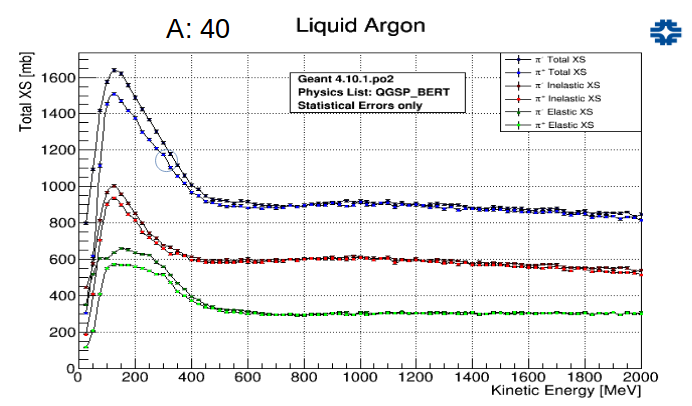
\includegraphics[scale=0.45]{./images/ArgonPionCrossSection.png}\\
\caption{$\pi$-Argon interaction cross-section generated using Geant4 (v4.10.1.po2) using the QGSP BERT model over the relevant kinetic energy range for LArIAT. See DocDB-1923 for more details.}
\label{fig:Geant4CrossSection}
\end{figure}

The pion interaction cross section depends on the mass of the target nucleus, as shown in Figure \ref{fig:Adep}, for different interaction channels near the $\Delta$-resonance region.

 
\begin{figure}[ht!]
\centering
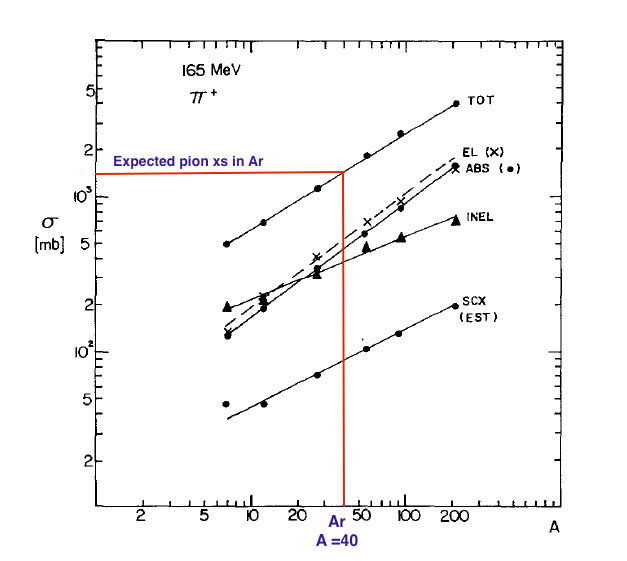
\includegraphics[scale=0.45]{./images/pionXS_vs_A.png}\\
\caption{Nuclear mass (A) dependence of $\pi^{+}$-nucleus interaction cross section for different interaction channels nearby the $\Delta$ resonance-region for 165 MeV/c pions.\cite{ashery1}}
\label{fig:Adep}
\end{figure}

Beyond intrinsic theoretical interest in nuclear structure, pion interactions play a critical role in understanding systematic uncertainties in neutrino experiments conducted at the GeV energy scale. Charged pions are produced in noticeable numbers in neutrino interactions with nuclei for neutrino energies of a few GeV.  

The interaction cross section of the pion strongly affects the possibility of detecting and measuring the pions. When pions are produced in $\nu$-Ar interactions, the inferred neutrino energy is based upon the measurement of the pion energies. Since the predicted pion cross section for interactions with nuclei is large, especially near the $\Delta$ resonance energy region, pion cross-sections can strongly impact the neutrino oscillation measurement. Thus, the precise measurement of the $\pi$-Ar interaction cross-section is important to future liquid argon neutrino experiments. In particular, current (MicroBooNE) and future (SBN and DUNE) neutrino oscillation experiments are very sensitive to pion cross section uncertainties. 

%%%%%%%%%%%%%%%%%%%%%%%%%%%%%%%%%%%%%%%%%%%%%%%%%%%%%%%%%
\subsection{Overview of the LArIAT Beamline}\label{sec:beamline}
%%%%%%%%%%%%%%%%%%%%%%%%%%%%%%%%%%%%%%%%%%%%%%%%%%%%%%%%%
The LArIAT experiment takes place at the Fermilab Test Beam Facility (FTBF) located in the Meson Building at Fermilab. A beam of 120~GeV protons is transported to the Meson Building and split to make two beam lines known as MCenter and MTest. LArIAT is served by the MCenter beam line, whose primary beam of 120~GeV protons impinges upon a thick target (25~cm) to create a secondary beam of charged particles, mainly pions, 8 - 80 GeV range. This collimated pion beam is momentum-selected and then transported the MC7 radiation enclosure, the LArIAT experiment hall.  

In the MC7 enclosure the secondary beam focuses onto a thick copper target and the resulting tertiary beam is collimated by a 1~m iron shield with an opening $-13\deg$ to beam's right with respect to the secondary beam direction. Two analyzing dipole magnets steer the beam path $+10\deg$, selecting a momentum window within 0.2 and 2.0~GeV/c and sign-selecting the particles and steering them to the TPC. The tertiary beam is instrumented with a pair of Time-of-Flight (TOF) scintillating detectors,  four Wire Chambers (WC) which allow measurement of each particle's momentum based on the location of the hits in the wire chambers, two Aerogel Cherenkov counters (AG) of different Cherenkov threshold to allow for $\mu / \pi$ separation, the LArTPC detector and a Muon Range Stack. Figure \ref{fig:beamlineschematic} gives a diagram of the tertiary beam line within the MC7 enclosure.

\begin{figure}[htb]
\begin{center}
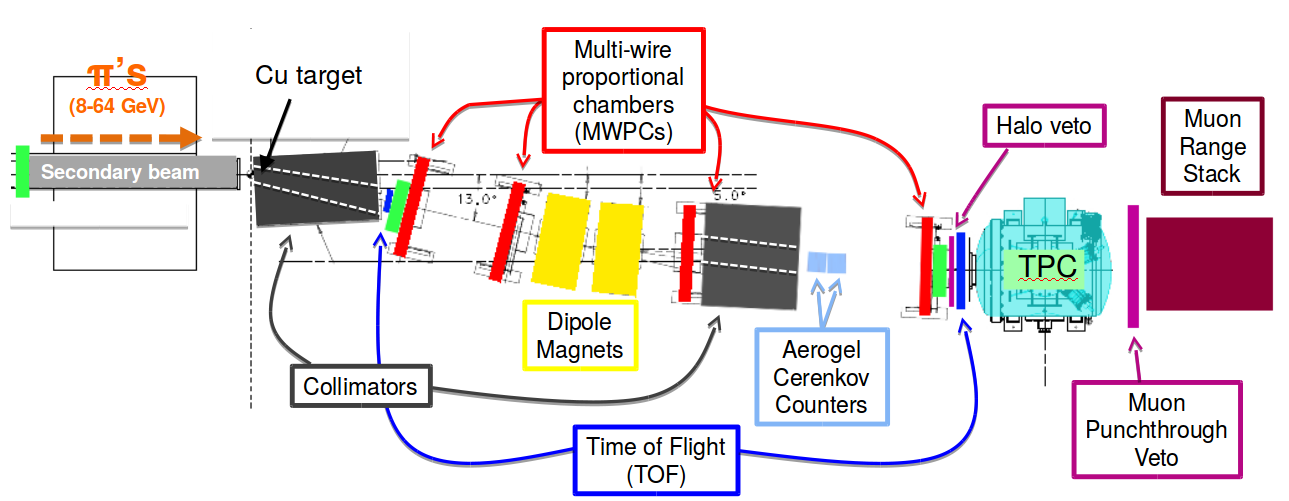
\includegraphics[scale=0.25]{./images/mc7beamline.png}
\end{center}
\caption{Schematic of the Tertiary Beam line within the MC7 enclosure.}
\label{fig:beamlineschematic}
\end{figure}

In this analysis, only the information from the Wire Chambers and the Time-of-Flight is used for particle identification. In particular, it is possible to calculate the mass of a given beamline track using the following equation

\begin{equation}
mass = \frac{p}{c}\sqrt{(\frac{TOF \times c}{l})^2 -1}
\end{equation}
where $p$ represents the measured momentum from the wire chamber, $TOF$ represents the time-of-flight measured as the difference between the two time-of-flight paddles in the LArIAT beamline, $l$ is path length the particle traveled down the beamline, and $c$ represents the speed of light. As is outlined in Section \ref{sec:EventSelection}, this allows us to select events based on the particle species.

%%%%%%%%%%%%%%%%%%%%%%%%%%%%%%%%%%%%%%%%%%%%%%%%%%%%%%%%%%%%%%%%%%%%%%%%%
\subsection{Beam composition}\label{sec:G4BeamlineMC}
%%%%%%%%%%%%%%%%%%%%%%%%%%%%%%%%%%%%%%%%%%%%%%%%%%%%%%%%%%%%%%%%%%%%%%%%%
The tertiary beam composition depends upon the energy of the secondary beam and the choice of magnetic field in the analyzing magnets. In Table \ref{tab:beamcomp1} and Table \ref{tab:beamcomp2} the beam composition is given in terms of percentage of different particle species per spill for negative and positive polarity. These are averaged values on several primary beam energies and magnets field intensities from MC simulations of the tertiary beam. As an example, the tertiary beam particle species and energy spectra for and negative polarity Monte Carlo and Data is shown in Figure \ref{fig:beamspectrum}  with 64 GeV of energy and the magnet setting of -100 T.

\begin{table}[ht!]
\centering
\begin{tabular}{|l|l|l|l|l|l|l|}
\hline
                      & $\pi^-$ & $e^-$ & $\gamma$ & $\mu^-$ & $K^-$ & $\overline{p}$ \\ \hline
Beam Composition (\%) &   48.4      &   40.9    &     8.5     &    2.2     &      0.035  &     0.007           \\ \hline
\end{tabular}
\caption{Beam Composition - Negative polarity configuration (from MC)}
\label{tab:beamcomp1}
\end{table}


\begin{table}[ht!]
\centering
\begin{tabular}{|l|l|l|l|l|l|l|}
\hline
                   & $\pi^+$ & $e^+$ & $\gamma$ & $\mu^+$ & $K^+$ & p \\ \hline
Beam Composition (\%) &    42.8     &  30.1     &    8.6      &    2.1     &    0.057    &    16.2            \\ \hline
\end{tabular}
\caption{Beam Composition - Positive polarity configuration (from MC)}
\label{tab:beamcomp2}
\end{table}



\begin{figure}[htb]
\begin{center}
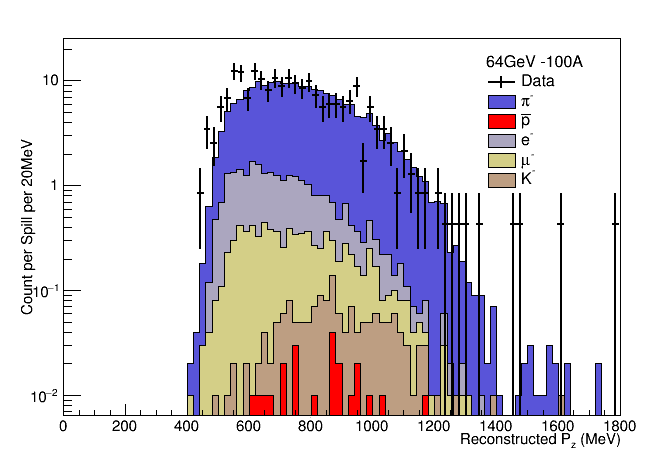
\includegraphics[scale=0.45]{./images/BeamSpectrumExample.png}
\end{center}
\caption{Tertiary Beam spectra for negative 100 Amp, 64 GeV target energy (from MC) with data overlayed.}
\label{fig:beamspectrum}
\end{figure}


%%%%%%%%%%%%%%%%%%%%%%%%%%%%%%%%%
%% SECTION 2: Data Samples
%%%%%%%%%%%%%%%%%%%%%%%%%%%%%%%%%
\section{Data / MC Samples}\label{sec:DataSamples}

This section outlines the data and Monte Carlo sets used in this analysis. For the data, we are using a set which spans all of Run-I and Run-II. The Monte Carlo uses the data momentum and angular spectrum to derive its initial conditions (known as Data Driven Monte Carlo: DDMC). The details of these samples and where they can be found are given in \href{https://docs.google.com/spreadsheets/d/1_0kNCKBIIx53f6vopqN2OijtcTICHD9rDvN_YKGH2mI/edit?usp=sharing}{this data production spreadsheet}


%%%%%%%%%%%%%%%%%%%%%%%%%%%%%%%%%%%%%%%%%%%%%%
\subsection{Data}\label{sec:data}
%%%%%%%%%%%%%%%%%%%%%%%%%%%%%%%%%%%%%%%%%%%%%%

The Run-I and Run-II data use the definitions \href{https://redmine.fnal.gov/redmine/projects/lardbt/wiki/Recommended_SAM_Datasets}{oulined on this Wiki page} and summarized in Table \ref{tab:datasamples}.

\begin{center}
\begin{table}[htb]
	\begin{center}
	%\resizebox{0.95\textwidth}{!}{%
	\begin{tabular}{|c|c|c|}
	\multicolumn{3}{c}{\textbf{Summary of Data Samples}} \\
	\hline \hline
	 Run Period & Data Set Definition & Samweb Meaning \\
	\hline
	 &  & \verb!defname: TPC_voltages_nominal! \\
	\hline
	 &  & \verb!TPC_MaxGainAndFilter! \\
	\hline
	Run-I & \verb!Lovely1_Neg_RunI_elenag_v02! & \verb!TPC_nominal_read_out_and_timing!  \\
	\hline
	 & & \verb!BothTOF_OnAndReadOut!  \\
	\hline
	 & & \verb!AllMWPC_OnAndReadOut!  \\
	 \hline
	 & & \verb!lariat_mid_f_mc7anb < 0! \\
	\hline
	\hline
	 & & \verb!run_number >= 8000 and run_number <= 10226! \\
    \hline	
	&  & \verb!defname: TPC_voltages_nominal! \\
	\hline
	 &  & \verb!TPC_MaxGainAndFilter! \\
	\hline
	Run-II & \verb!Lovely1_Neg_RunI_elenag_v03! & \verb!TPC_nominal_read_out_and_timing!  \\
	\hline
	 & & \verb!BothTOF_OnAndReadOut!  \\
	\hline
	 & & \verb!AllMWPC_OnAndReadOut!  \\
	 \hline
	 & & \verb!lariat_mid_f_mc7anb < 0! \\
	 \hline
	\end{tabular}%}
	\caption{Summary of the data samples used for this analysis. }
	\label{tab:datasamples}
	\end{center}
\end{table}
\end{center}

The relevant Samweb definitions listed in Table \ref{tab:datasamples} which require some explaining are defined as:

\begin{itemize}
\item \textbf{TPC Voltages Nominal}: Requires the cathode to be at greater than 23 kV, the collection plane wires voltage to be between 320 and 350 V, the induction plane voltage to be between -10 and -20 V, and the shield plane voltage to be greater than -310 V

\item \textbf{TPC MaxGainAndFilter}: Requires the ASIC configuration to be set as ``3'' for both the filter and the gain setting

\item \textbf{TPC Nominal Read Out and Timing}: Requires the readout of the TPC was enabled, the recorded number of time ticks is 3072, and the delay of 36900 was set on the v1495 (trigger card).


\end{itemize} 



%%%%%%%%%%%%%%%%%%%%%%%%%%%%%%%%%%%%%%%%%%%%%%%%%%%%%%%%%%%%
\subsection{Data $\pi/\mu/e$ Pre-selection}\label{sec:DataPreSelection}
%%%%%%%%%%%%%%%%%%%%%%%%%%%%%%%%%%%%%%%%%%%%%%%%%%%%%%%%%%%%
For each sample listed in Table \ref{tab:datasamples}, we outline the event selection used to select this data.

\begin{itemize}
\item \textbf{Time Stamp Filter}

A filter is used to select events which occurred in time with the beam. These events typically coincide with the first 6 seconds of the beam spill, and therefore the events are filtered using the following LArIATsoft settings

\begin{verbatim}
tfilt:      @local::lariat_timestampfilter

# ====================================================================
# Specify range of events to select.  For Run I/II:
#   - pedestal events:  ~ 0.  - 1.2 sec
#   - beam events:      ~ 1.2 - 5.5 sec
#   - cosmic events:    ~ > 5.5 sec
#   (default selects ALL events)
physics.filters.tfilt.T1:                       1.2
physics.filters.tfilt.T2:                       5.5
physics.filters.tfilt.RequireRawDigits:         true

\end{verbatim}



\item \textbf{Beamline Reconstruction}

The standard LArIAT beamline reconstruction is used to select events which have a wire chamber track and TOF information in an individual event using the following modules.
\begin{verbatim}
### beamline elements ###

wctrack:     @local::lariat_wctrackbuilder
tof:         @local::lariat_tof
agcounter:   @local::lariat_aerogel
\end{verbatim}


\textbf{For Run-I we use these default parameters:}
\begin{verbatim} 
physics.producers.wctrack.PickyTracks:                          false
physics.producers.tof.HitThreshold:                           -10.0  
physics.producers.tof.HitDiffMeanUS:                            0.6  
physics.producers.tof.HitDiffMeanDS:                            1.0  
physics.producers.tof.HitMatchThresholdUS:                      3.0  
physics.producers.tof.HitMatchThresholdDS:                      6.0  
physics.producers.tof.HitWait:                                  20.
\end{verbatim}

\textbf{For Run-II we use these default parameters:}
\begin{verbatim} 
physics.producers.wctrack.PickyTracks:                          false
physics.producers.tof.HitThreshold:                             -3.
physics.producers.tof.HitDiffMeanUS:                            0.5  
physics.producers.tof.HitDiffMeanDS:                            0.4  
physics.producers.tof.HitMatchThresholdUS:                      3.0  
physics.producers.tof.HitMatchThresholdDS:                      6.0  
physics.producers.tof.HitWait:                                  20.
\end{verbatim}

We do not require the tracks reconstructed in the wire chamber satisfy the criteria known as a ``picky track''. ``Picky tracks'' correspond to tracks reconstructed using hits in all four wire chambers. In these events, one and only one hit in each wire chamber track can be reconstructed per event and the track satisfies a straightness requirement in the Y-Z plane. These tracks have a slightly more accurate measure of the particle momentum than the ``high yield'' tracks which only require hits in three out of four of the wire chamber tracks and can have multiple wire chamber hits reconstructed per event but yield significantly better statistics. Details about wire chamber track reconstruction can be found in \cite{WCTrackReco}

\item \textbf{Particle Mass Filtering}
Using the beamline reconstruction, it is possible to calculate the mass of a given track, as shown in Figure \ref{fig:mass}. The classification of events into the different samples follows:

\begin{itemize}
\item \underline{$\pi, \mu, e$:} 0~MeV $<$ mass $<$ 350~MeV

\item \underline{kaon:} 350~MeV $<$ mass $<$ 650~MeV

\item \underline{proton:} 650~MeV $<$ mass $<$ 3000~MeV

\end{itemize}

\begin{figure}[htb]
\centering
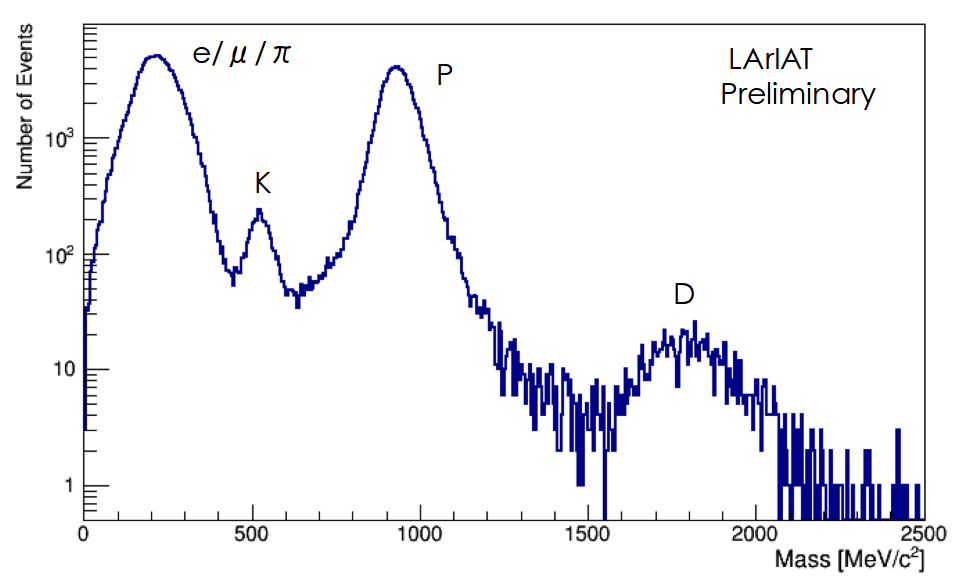
\includegraphics[width=0.70\textwidth]{images/mass.png}
\caption{The mass plotted for a sample of Run-II events reconstructed in the beamline. The classification of the events into $\pi, \mu, e$, kaon, or proton is based on this distribution.}
\label{fig:mass}
\end{figure}

For this analysis we require 0~MeV $<$ mass $<$ 350~MeV to select a sample of $\pi, \mu, e$ candidates for further event selection. The full event reduction table for these cuts is presented in Section \ref{sec:Results}.

\end{itemize}

%%%%%%%%%%%%%%%%%%%%%%%%%%%%%%%%%%%%%%%%%%%%%%%%%%%%%%%%%%%%
\subsection{Monte Carlo Samples}\label{sec:MCSamples}
%%%%%%%%%%%%%%%%%%%%%%%%%%%%%%%%%%%%%%%%%%%%%%%%%%%%%%%%%%%%
The precise details of how the Monte Carlo used in this study are given in \href{https://lartpc-docdb.fnal.gov:441/cgi-bin/ShowDocument?docid=2054}{docDB-2054} and  \href{https://lartpc-docdb.fnal.gov:441/cgi-bin/ShowDocument?docid=2056}{dobDB-2056}, a summary of which is presented here. 

The Data Driven Monte Carlo (DDMC) uses data quantities for a sample of Wire-Chamber tracks to derive the momentum ($P_x, P_y, P_z$) and angular $\theta, \phi$ distributions that are seen during a particular running period and/or running condition. Using those data derived distribution, in then launches single particle MC from $z = -100$~cm (the location of the fourth wire chamber) with these distributions as a template. An illustration of this procedure is shown in Figure \ref{fig:DDMC} with the results of the DDMC generation compared to a sample of wire chamber track data. Using this technique ensures the MC and data have very similar momentum and angular distributions initially and allow us to calibrate the energy loss upstream of the TPC as precisely as possible.

\begin{figure}[htb]
\centering
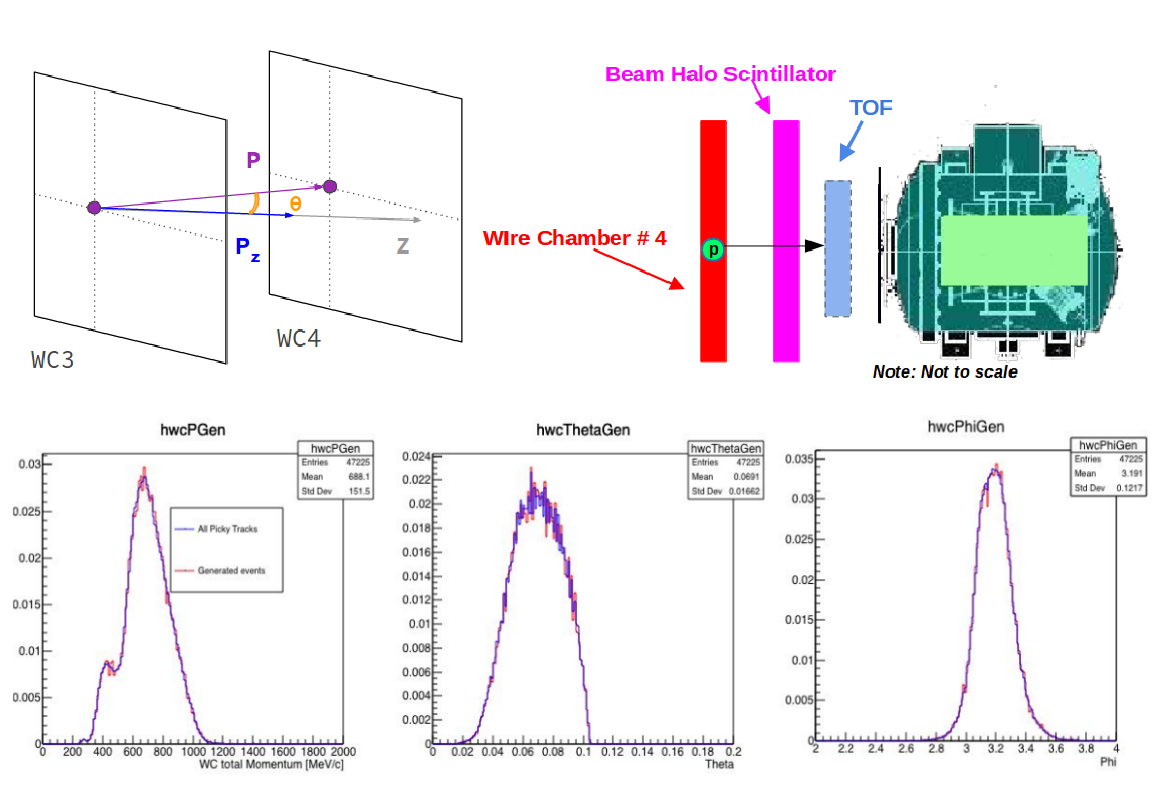
\includegraphics[width=0.70\textwidth]{images/DDMC.png}
\caption{Illustration of the technique where the wire chamber track initial angular and momentum distributions are used to generate the single particle MC.}
\label{fig:DDMC}
\end{figure}

Table \ref{tab:MCSampleGen} lists the various MC samples that were generated for this analysis. A sample of anti-protons was not generated for this analysis since they are estimated to make up less than $0.01\%$ of the overall sample.

\begin{table}[htb]
	\begin{center}
	\resizebox{0.95\textwidth}{!}{%
	\begin{tabular}{|c|c|c|}
	\hline
	  \textbf{DDMC Sample} & Original Data Distribution & Number of Events Generated  \\
	Run-I $\pi^{-}$ & $\pi, \mu, e$ Mass Filter / High Yield WC-Track & 358,000 \\
	\hline
	Run-I $\mu^{-}$ & $\pi, \mu, e$ Mass Filter / High Yield WC-Track &  \\
	\hline
	Run-I $e^{-}$ & $\pi, \mu, e$ Mass Filter / High Yield WC-Track & 359,000\\
	\hline
	Run-I $K^{-}$ & $K^{-}$ Mass Filter / High Yield WC-Track & \\
	\hline
	\hline
	Run-II $\pi^{-}$ & $\pi, \mu, e$ Mass Filter / High Yield WC-Track & 360,000\\
	\hline
	Run-II $\mu^{-}$ & $\pi, \mu, e$ Mass Filter / High Yield WC-Track & 361,000 \\
	\hline
	Run-II $e^{-}$ & $\pi, \mu, e$ Mass Filter / High Yield WC-Track & 359,000\\
	\hline
	Run-II $K^{-}$ & $K^{-}$ Mass Filter / High Yield WC-Track & \\
	\hline
	\end{tabular}}
	\caption{Summary of MC generated for the analysis.} \label{tab:MCSampleGen}
	\end{center}
\end{table}

In addition to this sample of DDMC, a sample of photons is also generated since as is shown in Table \ref{tab:beamcomp1} a small but non-negligible portion of the beam will have photons entering the TPC. This sample is generated with a flat momentum spectrum between 0 MeV and 2000 MeV with a Gaussian angular distribution of $\pm$5 degrees about the beam direction. The photon momentum spectrum is then re-weighted by the momentum spectrum of the corresponding run period it is being simulated for. This approximation allows us to estimate the contamination due to photons from MC with a reasonable assumption of their spectrum.


%%%%%%%%%%%%%%%%%%%%%%%%%%%%%%%%%
%% SECTION 3
%%%%%%%%%%%%%%%%%%%%%%%%%%%%%%%%%
\newpage
\section{Inclusive $\pi$ Analysis}\label{sec:PionAnalysis}

In this section we will give an overview of the $\pi^{-}$-inclusive cross-section analysis specific cuts as well as a summary of the ``thin-slice'' method used to extract the inclusive cross-section.


%%%%%%%%%%%%%%%%%%%%%%%%%%%%%%%%%%%%%%%%%%%%%%%%%%%%%%%
\subsection{Overview of Pion TPC Candidate ID}\label{sec:TPCCandidateSelect}
%%%%%%%%%%%%%%%%%%%%%%%%%%%%%%%%%%%%%%%%%%%%%%%%%%%%%%%
Wherever possible, data and Monte Carlo are treated identically for the analysis specific cuts. The selection criteria were developed for this analysis to identify events in which the measured $\pi, \mu, e$ candidate track from the beamline could be matched to activity within the LArTPC. Selections are made to allow disambiguating the activity in the TPC and matching this to the beamline track as well as attempting to reject activity which comes from electromagnetic showers (e.g. electrons and photons) in the beamline.

\begin{itemize}
\item{\textbf{Require the presence of a track in the upstream portion of the TPC}}\\

To select events which can be well matched to the reconstructed WC-track, we require at least one of the TPC reconstructed tracks to have a spacepoint within the first 2 cm in z coordinate, as shown in Fig.\ref{fig:UsFilter0}. An event is rejected if none of the reconstructed tracks have a space point with $0 < z < 2$ cm. The choice of 2~cm distance was arrived at from MC studies outlined in \href{https://lartpc-docdb.fnal.gov:441/cgi-bin/ShowDocument?docid=1766}{docDB-1766} , \href{https://lartpc-docdb.fnal.gov:441/cgi-bin/ShowDocument?docid=1778}{docDB-1778}, \href{https://lartpc-docdb.fnal.gov:441/cgi-bin/ShowDocument?docid=1784}{docDB-1784}

\item{\textbf{Track Multiplicity Requirement}}\\
To reduce both the number of events with high pile-up as well as to reject events which have an electromagnetic shower developing early in the upstream portion of the TPC, we filter events based on the number of tracks present in the region from 0~cm<$z$<14~cm. If more than three tracks are found in this region, the event is removed. The region 0~cm<$z$<14~cm and the requirements of less than four tracks was chosen by comparing pion MC to electron/photon MC as well as looking at a preliminary sample of data (as outlined in \href{https://lartpc-docdb.fnal.gov:441/cgi-bin/ShowDocument?docid=1766}{docDB-1766} , \href{https://lartpc-docdb.fnal.gov:441/cgi-bin/ShowDocument?docid=1778}{docDB-1778}, \href{https://lartpc-docdb.fnal.gov:441/cgi-bin/ShowDocument?docid=1784}{docDB-1784})

\item{\textbf{Shower Rejection}}\\

Hand-scanning a sample of data from Run-I it was found that after applying the selection criteria previously mentioned, there remained a significant sample of residual electromagnetic showers aligned with beam (see Figure \ref{fig:stillShow}). 

\begin{figure}[h!]
\centering
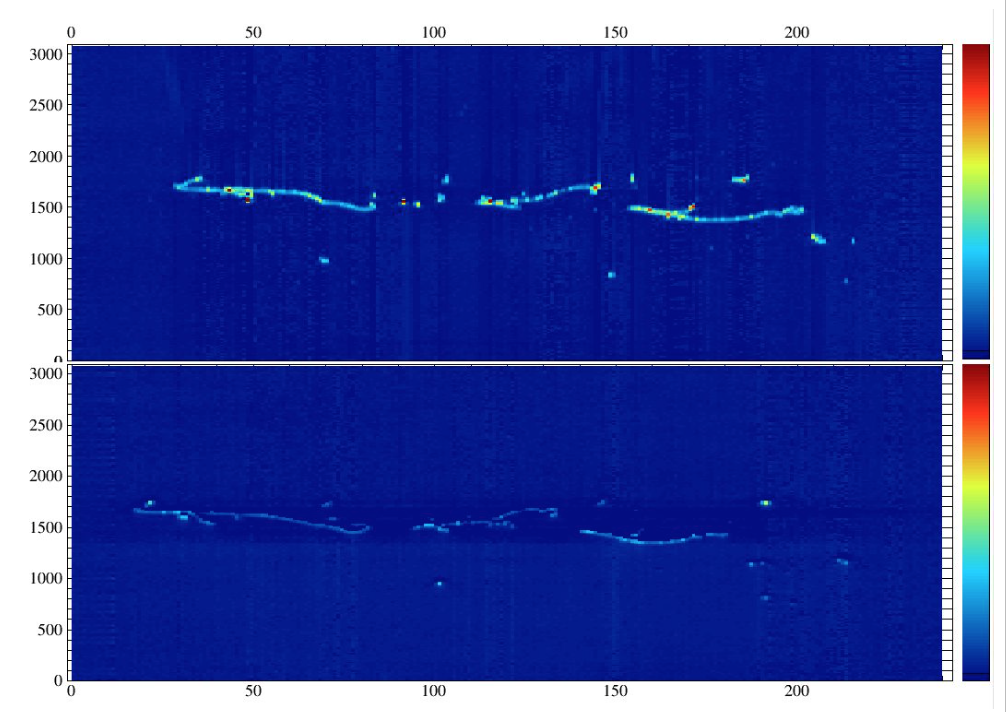
\includegraphics[scale=0.45]{./images/showerEvent.png}
\caption{Example of a "shower-like" event that passes all the previous selection cuts.}
\label{fig:stillShow}
\end{figure}

To eliminate events like this we utilize a simple ``track-based'' filter which, as shown from MC studies, removes a large number of electromagnetic events while still keeping pion events. 

This filter evaluates how many tracks in the TPC are reconstructed for the event and the length for each of these tracks. We then count how many of those tracks would be classified as "short tracks" where ``short'' is any track with length less than 5 cm. Events with more than two ``short'' tracks are removed from consideration. Figure \ref{fig:showrej} shows a graphical representation of this shower based event filter.

\begin{figure}[h!]
\centering
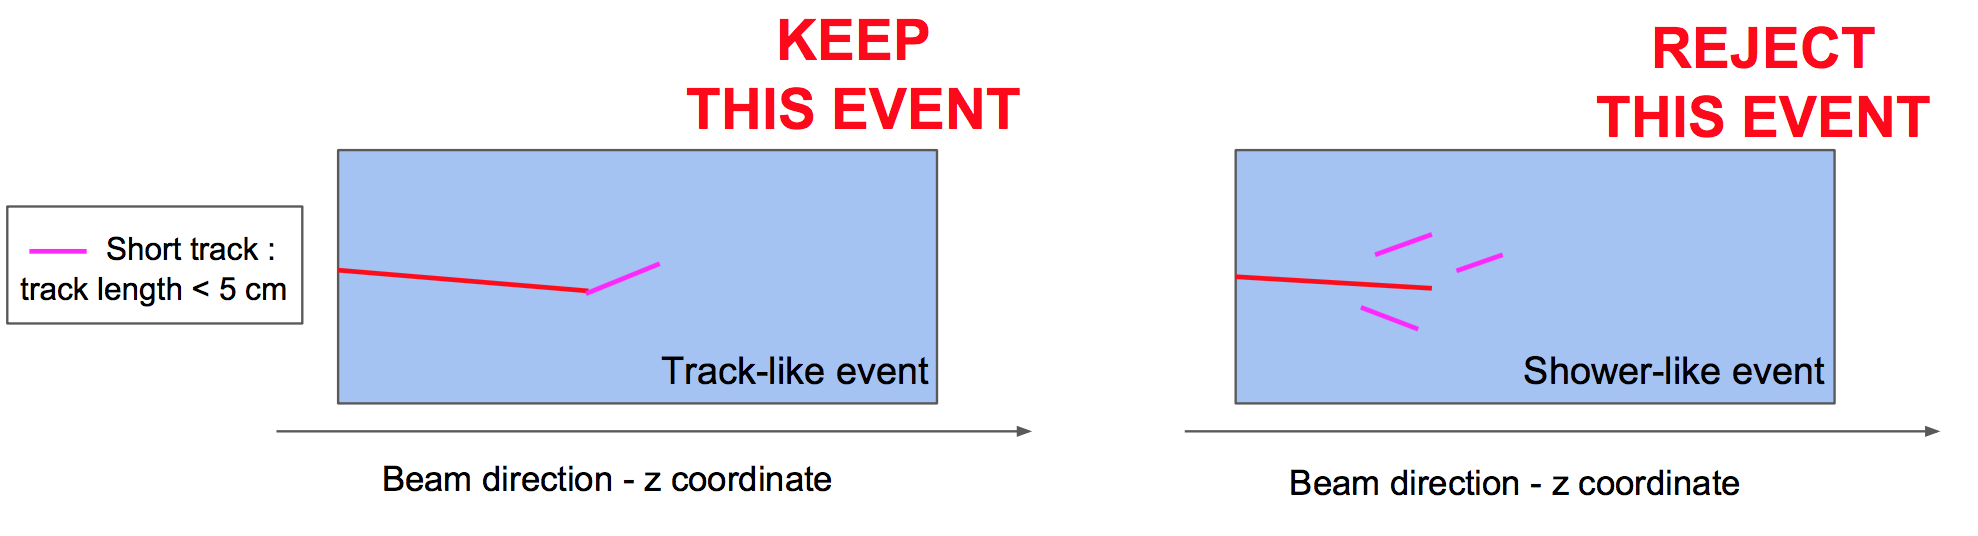
\includegraphics[scale=0.45]{./images/ShowerRejection.png}
\caption{Representation of the Residual Showers Rejection cut.}
\label{fig:showrej}
\end{figure}

The number of ``short'' tracks and the length of the tracks has been chosen utilizing a preliminary scan of the open box data sample and comparing the values to the single particle Monte Carlo attempting to maximize our signal compared to the background.

\item{\textbf{WC to TPC Track Match}}\\

We attempt to uniquely match one WC-Track to one and only one reconstructed TPC track. This match is done to the upstream most point of the TPC track by matching in the $X$ and $Y$ coordinate of the extrapolated WC-Track to the upstream most point of the reconstructed TPC Track as well as matching the incoming track angle to the reconstructed TPC track angle.

We define $\Delta$X as the difference between the $x$ position of the most upstream point of the TPC track and the $x$ position of the WC track as projected to the TPC front face. $\Delta$Y is defined analogously. $\Delta\alpha$ is the angle between the incident WC Track and the TPC track in the plane that contains them. If a Wire Chamber Track to TPC match is found with a  -4~cm~$< \Delta X<$ 6~cm, -5~cm $ < \Delta Y< $~5~cm, and $\alpha < $ 10$^o$ then we consider this a ``well matched'' track. We require each event to have one and only one well matched WC-Track/TPC Track pair.

\begin{figure}[h!]
\centering
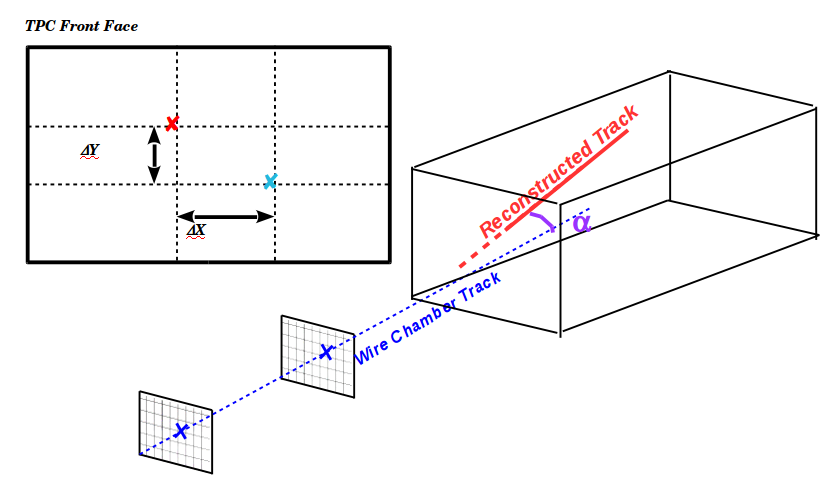
\includegraphics[scale=0.35]{./images/WCTPCMatchSchematic.png}
\caption{Schematic which shows the matching between Wire Chamber tracks and TPC tracks (top) as well as MC particles and TPC tracks.}
\label{fig:WCTrackMatching}
\end{figure}

In the Monte Carlo, there is no reconstructed WC-Track, so instead a projected track from the point of generation is made simulate the WC-Track. The reconstructed MC-track is then matched to this projected point at the front face of the TPC. While this method does not capture the efficiency associated with the wire chamber track algorithm itself, it does allow for a matching based on the data topology and momentum.

\end{itemize}

Having now developed the method by which we select the pion candidate track and have this track uniquely matched to a wire chamber track, we can proceed with analyzing this to establish the cross-section. In order to do this, it is necessary to lay out the general technique used in this analysis.

%%%%%%%%%%%%%%%%%%%%%%%%%%%%%%%%%%%%%%%%%%%%%%%%%%%%%%%%%
\subsection{Thin slice method}\label{sec:ThinSlice}
%%%%%%%%%%%%%%%%%%%%%%%%%%%%%%%%%%%%%%%%%%%%%%%%%%%%%%%%%
In general, the target is not a single particle, but a slab of material containing many diffusion centers. If we assume the target centers to be uniformly distributed in the material and the target to be thin enough not to have one center sitting in front of another, we are in the so-called  "thin target" approximation. A pictorial representation of the ``thin slice'' approximation is shown schematically in Figure \ref{fig:thinslice}


\begin{figure}[htb]
\centering
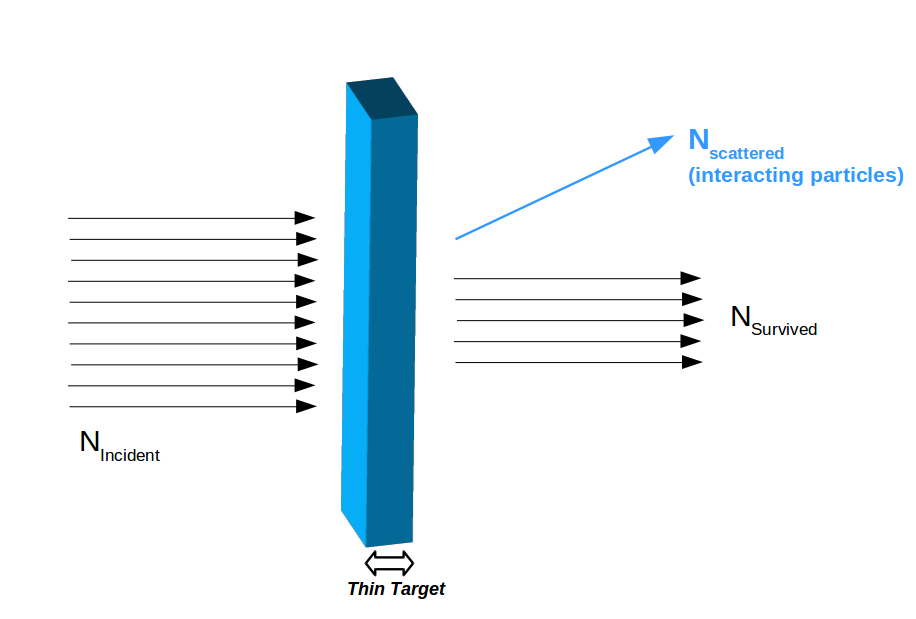
\includegraphics[scale=0.25]{./images/ThinTarget.png}
\caption{Representation of the thin target approximation as a ``thin slice'' of argon.}
\label{fig:thinslice}
\end{figure}

The survival probability of a pion traveling through a slab of argon of depth {\it z} and density {\it n} is given by

\begin{equation}
P_{survival} = e^{-\sigma_{total}n z},
\end{equation} 

where $\sigma_{tot}$ is the total cross section per nucleon (in $cm^2$). Then the interaction probability is given by one minus the survial probability
\begin{equation}
P_{interacting} = 1 - P_{survial}.
\end{equation}
Experimentally we can measure interaction probability ($P_{interacting}$) by measuring the ratio of the number of interacting pions to the number of incident pions, $N_{interacting}/N_{incident}$ for a given slab at a given energy:

\begin{equation}\label{eqn:ProbInteraction}
P_{interacting}=\frac{N_{interacting}}{N_{incident}}=1-e^{-\sigma_{tot}n z}
\end{equation}

By expanding Equation \ref{eqn:ProbInteraction} (assuming a small $z$ slab) the probability of interacting can be expressed as

\begin{equation}
P_{interacting} = 1 - (1-\sigma_{total}n z \delta + ...).
\end{equation}

Rearranging this expression, the measured rate of interactions can be used to calculate the total cross section as a function of energy
\begin{equation}\label{calc_sigma}
\sigma_{tot}(E) \simeq \frac{1}{nz} \Big(\frac{N_{interacting}}{N_{incident}}\Big) 
\end{equation}
where {\emph{z}} is the target thickness (in cm) along the incident pion direction, and {\emph{n}} is the scattering center density in the target, $n=\frac{\rho N_{A} }{A}$ (in $cm^{-3}$). 

The uncertainty for each energy bin is calculated by error propagation from the uncertainty on $N_{incident}$ and $N_{interacting}$. 
Since the number of incident pions in each slice is given by a simple counting, it is safe to assume that $N_{incident}$ is distributed as a poissonian with mean and $\sigma^2$ equal to $N_{incident}$ in each bin.  
On the other hand, $N_{interacting}$ follows a binomial distribution: the particle in a given energy bin might or might not interact.  The interaction probability $p$ is $\frac{ N_{interacting}}{N_{incident}}$ and the number of tries $n$ is $N_{incident}$. 
So, the square of the variance for the binomial is given by  $$\sigma^2 = np(1-p) =  N_{incident}\frac{ N_{interacting}}{N_{incident}} (1-\frac{ N_{interacting}}{N_{incident}}) = N_{interacting}(1-\frac{ N_{interacting}}{N_{incident}}).$$

$N_{incident}$ and $N_{interacting}$ are not independent.
The uncertainty on the cross section is thus calculated as 
\begin{equation}
\delta\sigma_{tot}(E) = \sigma_{tot}(E) \Big(\frac{\delta N_{interacting}}{N_{interacting}}+\frac{\delta N_{incident}}{N_{incident}}\Big) 
\end{equation}
where:
\begin{eqnarray}
\delta N_{incident} = \sqrt[]{N_{incident}} \\
\delta N_{interacting} = \sqrt[]{N_{interacting}(1-\frac{ N_{interacting}}{N_{incident}})}.
\end{eqnarray}

%%%%%%%%%%%%%%%%%%%%%%%%%%%%%%%%%%%%%%%%%%%%%%%%%%%%%%%%%%%%%%%%%%%%%%%%%%
\subsection{Thick Target Method - Slicing the LArTPC in thin targets}
%%%%%%%%%%%%%%%%%%%%%%%%%%%%%%%%%%%%%%%%%%%%%%%%%%%%%%%%%%%%%%%%%%%%%%%%%% 

When the "thin target" approach is not applicable, such as in the case of "thick target" experiments like LArIAT, a slightly different technique is needed in order to accurately evaluate the pion cross section dependence on energy. In particular, one must know the energy loss of the pion as it crosses the "thick" target before reaching its interaction point. In the ``thin slice'' approximation it is reasonable to only consider the $\pi$-nucleus hadronic interactions, while for the "thick" target case, it is necessary to take into account other pion interactions such as pion decay (both in flight and at rest) as well as pion capture at rest on the target nuclei.

A new technique, called the "sliced TPC" method, was developed in order to make the measurement possible in the thick target LArTPC~\cite{myThesis} environment. The fine-grained tracking of the LArIAT LArTPC allows us to treat the 90-cm thick LAr volume as a sequence of many adjacent thin targets. 

For LArIAT, the two wire planes are each composed of 240 wires oriented at +/- $60^{\circ}$ at 4 mm spacing. The wires collect signals proportional to the energy loss of the pion in a $60^{\circ}$-inclined 4~mm thin slab of liquid argon. Thus, one can think of the TPC as being subdivided into many slices of $\Delta${\emph{z}} = 4 mm/sin($60^{\circ}$) $\approx$ 4.5~mm thickness along the {\emph{z}} axis, i.e., direction of the incident particles (pions), as shown in Fig.~\ref{fig:slicedtpc}. 

Each slice {\emph{n}} can be now considered as a "thin target" and we can apply the cross section calculation from Eq.~\ref{calc_sigma} iteratively, evaluating the actual kinetic energy of the pion as it enters each slice, $E_{n}^{kin}$. The energy of the pion entering the TPC is known by the momentum determination of the tertiary beamline, and the incident energy of the pion at the successive slab is determined by subtraction of the calorimetric energy released by the particle in the previous slab. If the particle enters a slice, it contributes to $N_{incident}$ in the energy bin corresponding to its kinetic energy in that slice. If it interacts in the slice, it then also contributes to $N_{interacting}$ in the appropriate energy bin.

%\textcolor{blue}{Sketch of sliced tpc technique?}
\begin{figure}[ht!]
\centering
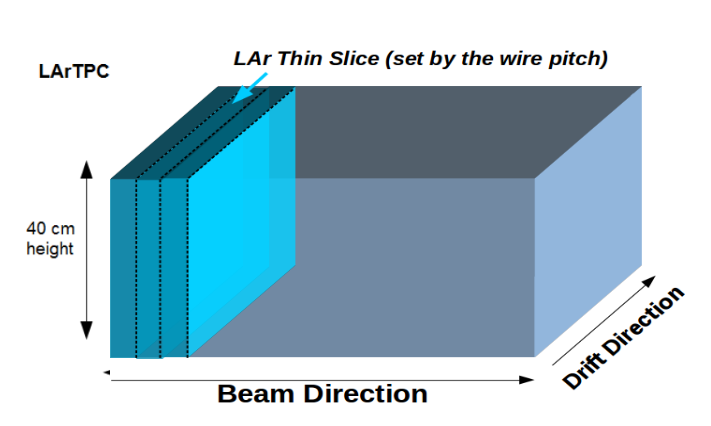
\includegraphics[scale=0.35]{./images/SlicedTPC.png}\\
\caption{Sketch of Sliced TPC approach.}
\label{fig:slicedtpc}
\end{figure}

The "sliced TPC" technique was tested by comparing the results of this method with the prediction of the total hadronic interaction cross section ($\pi^{\pm}$, Ar) for thin-target simulations from two Monte Carlo generators (Geant 4.10.1 with Bertini Cascade model~\cite{geant4, g4bert} and Genie v2.8.2 with intranuke-hA model). The thick target simulation used a simple stand-alone Geant4 simulation  (i.e., no other detector features were taken into account except the geometry of the thin slices in the LAr volume). Fig.~\ref{fig:xsplot} shows the resulting total ${\pi^-}$ cross section extracted by the sliced TPC technique; it agrees well with the Geant 4 thin-target cross section. The Genie thin-target cross section for $^{40}$Ar shown in this figure is significantly different than that of Geant at low kinetic energies due to the fact that Geant4 models are tuned on $^{12}$C while Genie ones are tuned on a much heavier $^{56}$Fe target. The extrapolated cross section predicted for $^{40}$Ar can be then very different, especially in the resonance region where the model is strongly target-dependent from one generator to another.
 
The comparison of the Geant4 thin- and thick-target cross section results demonstrates the power of the "sliced TPC" method for the measurement of the ($\pi^{\pm}$, Ar) cross section in LArIAT TPC geometry. 

\begin{figure}[h!]
\centering
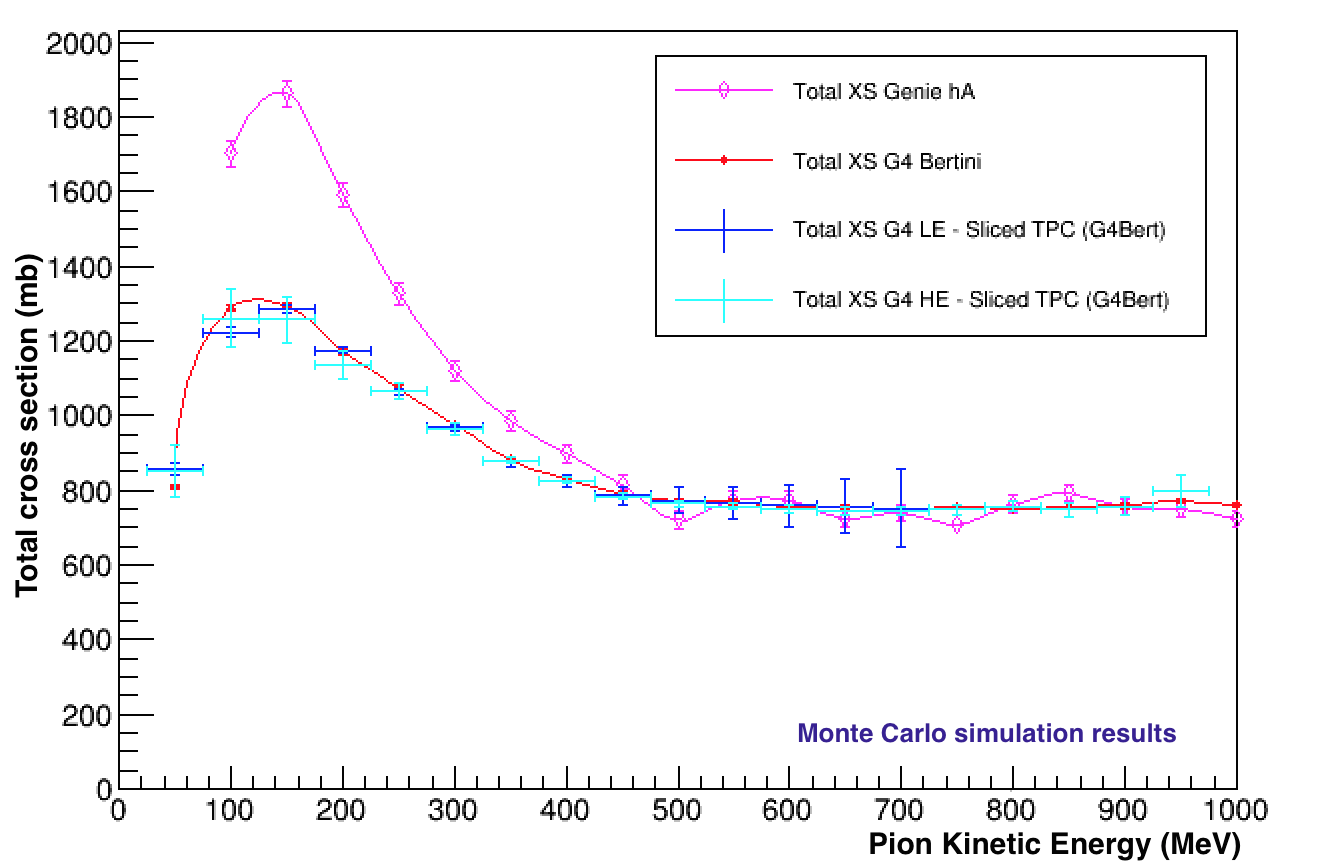
\includegraphics[scale=0.45]{./images/compare_new.png}
\caption{$\pi^-$ on Ar total cross section dependence on the kinetic energy from MC simulations: comparison between Geant4 and Genie predictions for a LAr thin target and extrapolated cross section with the ``Sliced TPC'' approach with a Geant4 Bertini based simulation of the LArTPC thick target \cite{myThesis}.}
\label{fig:xsplot}
\end{figure}

Having validated the ``Sliced TPC'' technique and shown that the this technique recovers the simulated cross-section, we now move to performing this measurement utilizing the complete LArIAT simulation within the LArSoft \cite{} based simulation.  Furthermore, we move from utilizing particle level MC-truth information to performing fully automated reconstruction of the charged pion events within the LArTPC. 







%%%%%%%%%%%%%%%%%%%%%%%%%%%%%%%%%
%% SECTION 4
%%%%%%%%%%%%%%%%%%%%%%%%%%%%%%%%%
%%\section{\textcolor{blue}{R\&D Strategy}}
%\section{Results}\label{sec:Results}
In this section we overview the results of the event selection outlined in the previous sections. Section \ref{sec:DataReduction} gives the breakdown of data events passing all our selection cuts and presents the beamline plots for this sample. Section \ref{sec:MCReduction} provides the similar breakdown of the MC events passing the selection cuts. Section \ref{sec:ValidationPlots} overviews a series of Data/MC comparisons to validate that the sample of simulated events is well reproduced in the data. Finally, Section \ref{sec:CrossSection} shows the inclusive $\pi^{-}$-Argon cross-section.


%%%%%%%%%%%%%%%%%%%%%%%%%%%%%%%%%%%%%%%%%%%%%%%%%%%
\subsection{Data Event Reduction} \label{sec:DataReduction}
%%%%%%%%%%%%%%%%%%%%%%%%%%%%%%%%%%%%%%%%%%%%%%%%%%%
Table \ref{tab:CutSummary} gives the event reduction for the negative polarity $\pi, \mu, e$ data sample for Run-I, Run-II, and combined. The definition of the cuts presented here are given in Section \ref{sec:TPCCandidateSelect}

%%% Put event reduction tables here 
\begin{table}[htb]
	\begin{center}
	\resizebox{0.95\textwidth}{!}{%
	\begin{tabular}{|c|c|c|c|}
	\hline
	%\multicolumn{5}{|c|}{\textbf{Summary of inclusive NC $\pi^{0}$ Event Selection Cuts}} \\
	%\hline \hline
	  \textbf{Event Selection} & Run-I Negative Polarity & Run-II Negative Polarity & Combined  \\
	\hline
	Total Number of Beam Events & 113,336 & 1,585,598 & 1,698,934 \\
	\hline
	$\pi, \mu, e$ Mass Selection & 20,653 & 493,455 & 514,108 \\
	\hline
	20~ns $<$TOF$<$27 & 20,577 & 485,159 & 505,736 \\
	\hline
	Requiring an upstream TPC Track within $z<2$cm & 18,882  & 403,561   &  422,443 \\
	\hline
	$<4$ tracks in the first $z<14$cm & 12,910  & 316,451  & 329,361 \\
	\hline
	Electromagnetic shower rejection & 9,824  & 232,510  &  242,334 \\
	\hline
	Unique match between WC/TPC Track & 5,500 & 120,956 & 126,456\\
	\hline
	\hline
	\end{tabular}}
	\caption{Summary of the events passing the inclusive pion selection criteria.} \label{tab:CutSummary}
	\end{center}
\end{table}

For the combined Run-I/Run-II sample Figures \ref{fig:WCandTOFBeamlinePlot}, \ref{fig:DeltaXDeltaY} show the time-of-flight and momentum spectrum as well as the results of the WC/TPC matching. The addition of a cut on the TOF to require  20~ns $<$TOF$<$27 is to clean up the low momentum high TOF events seen in Figure \ref{fig:WCandTOFBeamlinePlot}.

\begin{figure}[h!]
\centering
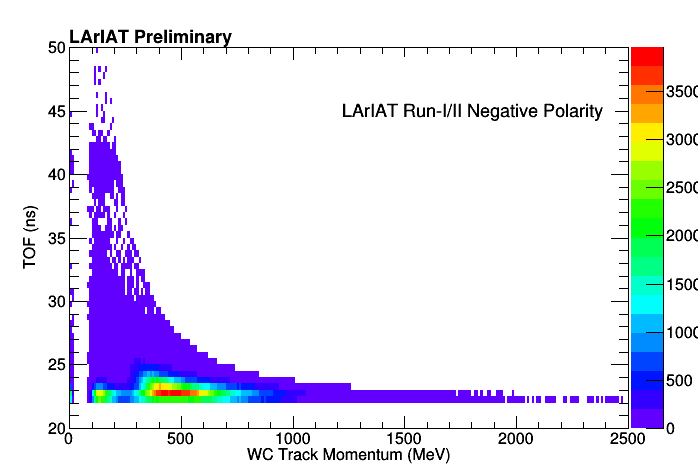
\includegraphics[scale=0.30]{./images/TOFvsWCTrk.png}
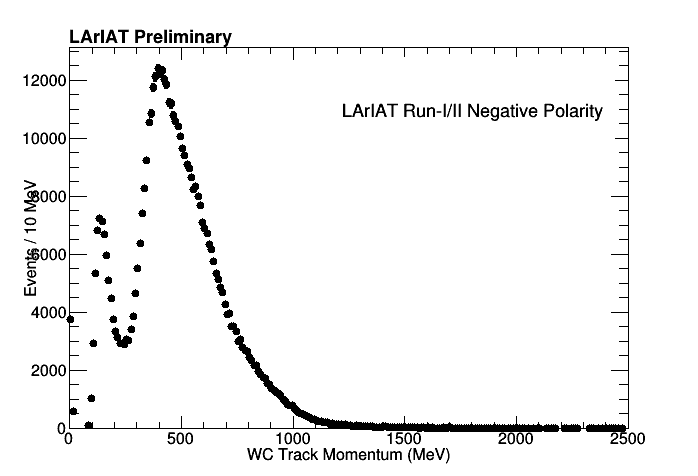
\includegraphics[scale=0.30]{./images/wctrkMomentum.png}
\caption{(Left) Time-of-Flight vs Wire Chamber Track Momentum. (Right) The momentum spectrum for our sample.}
\label{fig:WCandTOFBeamlinePlot}
\end{figure}

\begin{figure}[h!]
\centering
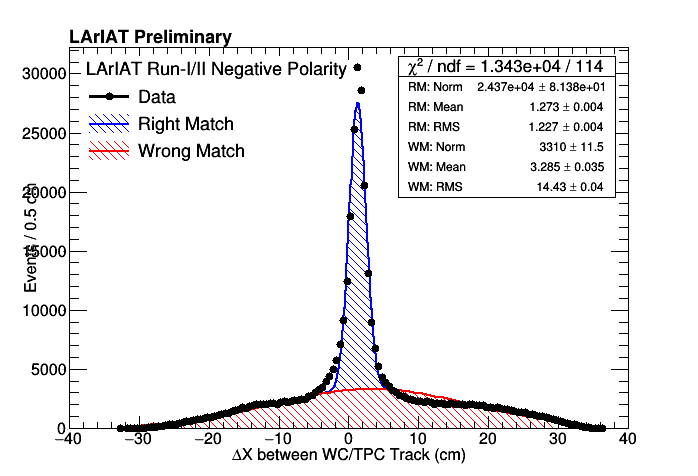
\includegraphics[scale=0.30]{./images/DeltaX.png}
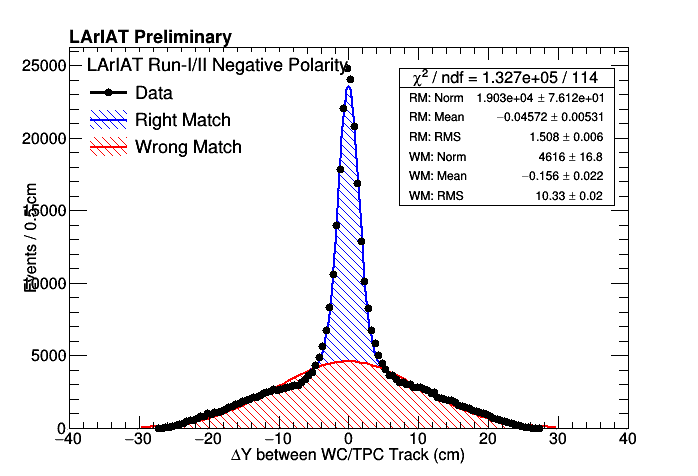
\includegraphics[scale=0.30]{./images/DeltaY.png}
\caption{The $\Delta X$ and $\Delta Y$ distributions prior to requiring the match between the TPC and WC track.}
\label{fig:DeltaXDeltaY}
\end{figure}

%%%%%%%%%%%%%%%%%%%%%%%%%%%%%%%%%%%%%%%%%%%%%%%%%%%
\subsection{MC Event Reduction} \label{sec:MCReduction}
%%%%%%%%%%%%%%%%%%%%%%%%%%%%%%%%%%%%%%%%%%%%%%%%%%%
Table \ref{tab:MCRunIICutSummary} shows a similar event reduction as was done in previous section for the sample of Run-II MC.

%%% Put event reduction tables here 
\begin{table}[htb]
	\begin{center}
	\resizebox{0.98\textwidth}{!}{%
	\begin{tabular}{|c|c|c|c|c|c|}
	\hline
	%\multicolumn{5}{|c|}{\textbf{Summary of inclusive NC $\pi^{0}$ Event Selection Cuts}} \\
	%\hline \hline
	  \textbf{Event Selection} & Run-II High Yield & Run-II High Yield & Run-II High Yield & Run-II High Yield & Run-II High Yield \\
	   & $\pi^{-}$ MC & $\mu^{-}$ MC  & $e^{-}$ MC & $K^{-}$ MC & $\gamma$ MC \\
	\hline
	Total Number of MC Events & 359,000 & 361,000 & 361,000 & 185,000 & 193,500 \\
	\hline
	MC-Particle Reaches the TPC & 245,511 & 246,874 & 323,997 & 95,391 & 72,782 \\
	\hline
	Requiring an upstream TPC Track within $z<2$cm & 220,752 & 221,966 & 254,218 & 82,407 & 5,782 \\
	\hline
	$<4$ tracks in the first $z<14$cm & 220,454 & 221,666 & 239,406 & 81,369 & 5,730 \\
	\hline
	Electromagnetic shower rejection & 218,068 & 219,274 & 94,293 & 77,281 & 2,471 \\
	\hline
	Unique match between WC/TPC Track & 180,341 & 181,327 & 46,133 & 67,420 & 1,670\\
	\hline
	\hline
	\end{tabular}}
	\caption{Summary of the MC events passing the inclusive pion selection criteria.} \label{tab:MCRunIICutSummary}
	\end{center}
\end{table}

Since the data has significantly more statistics for Run-II compared to Run-I ($\sim$22:1 ratio), the Run-II MC is used for the purposes of comparison as mixing of the two samples in this ratio does not change the final result. For the sake of completeness, Table \ref{tab:MCRunICutSummary} shows a similar event reduction as was done in previous section for the sample of Run-I MC.

%%% Put event reduction tables here 
\begin{table}[htb]
	\begin{center}
	\resizebox{0.95\textwidth}{!}{%
	\begin{tabular}{|c|c|c|c|c|c|}
	\hline
	%\multicolumn{5}{|c|}{\textbf{Summary of inclusive NC $\pi^{0}$ Event Selection Cuts}} \\
	%\hline \hline
	  \textbf{Event Selection} & Run-I High Yield & Run-I High Yield & Run-I High Yield & Run-I High Yield & Run-I High Yield \\
	   & $\pi^{-}$ MC & $\mu^{-}$ MC  & $e^{-}$ MC & $K^{-}$ MC & $\gamma$ MC \\
	\hline
	Total Number of MC Events & 357,000 &  &  & & 193,500 \\
	\hline
	MC-Particle Reaches the TPC & 258,294 &  &  & & 72,782 \\
	\hline
	Requiring an upstream TPC Track within $z<2$cm & 233,763  &  &  & & 5,782 \\
	\hline
	$<4$ tracks in the first $z<14$cm & 233,447  &  &  & & 5,730 \\ 
	\hline
	Electromagnetic shower rejection & 230,960  &  & & & 2,471 \\
	\hline
	Unique match between WC/TPC Track & 189,670 &  & & & 1,670\\
	\hline
	\hline
	\end{tabular}}
	\caption{Summary of the MC events passing the inclusive pion selection criteria.} \label{tab:MCRunICutSummary}
	\end{center}
\end{table}

Table \ref{tab:MCPercentageTable} summarizes the fraction of events passing all the inclusive pion analysis cuts. This fraction is calculated using the number of events passing all the cuts divided by the number of MC events which reach the front face of the TPC. We use the number of MC events reaching the front face of the TPC instead of the total number of MC events because using the latter would mis-represent the efficiency of the TPC based cuts.

\begin{table}[h!]
\centering
\resizebox{0.95\textwidth}{!}{%
\begin{tabular}{|c|c|c|c|c|c|}
\hline
 & $\pi^{-}$ MC & $\mu^{-}$ MC  & $e^{-}$ MC & $K^{-}$ MC & $\gamma$ MC \\
\hline
\textbf{Percent of events passing cut} & 73.5$\%$ & 73.4$\%$ & 14.2 $\%$ & 70.6$\%$ & 2.3$\%$ \\
\hline
\end{tabular}}
\caption{Fraction of MC Events passing inclusive pion analysis cuts.}
\label{tab:MCPercentageTable}
\end{table}

It should also be noted that the efficiency for selecting $K^{-}$ events is likely to be overly inflated here both because they make up a very small percentage of the negative polarity beam $< 1\%$ and because these cuts do not take into account the beamline mass filter applied to the data.

Figure \ref{fig:TrueInteractionTypes} shows the breakdown of $\pi^{-}$-Argon interaction types as a function of true kinetic energy taken from the pion DDMC. One important feature of this plot to note that pion capture-at-rest dominates. This process is not one which should be included in the total $\pi^{-}$-Argon interaction cross-section.

\begin{figure}[h!]
\centering
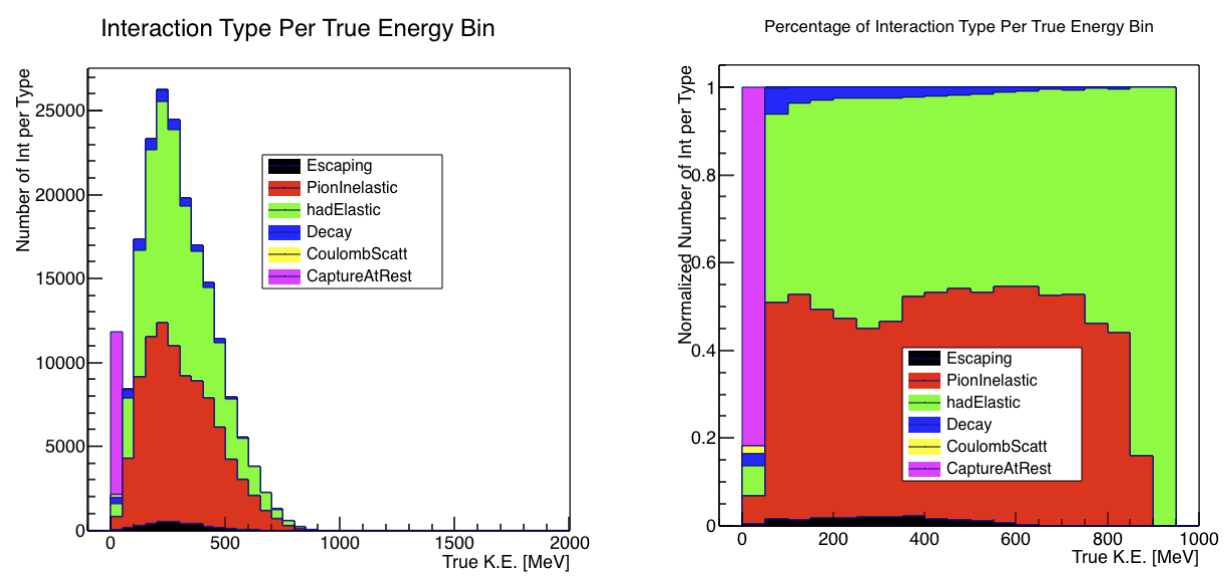
\includegraphics[scale=0.33]{./images/PiArIntTypesTrue.png}
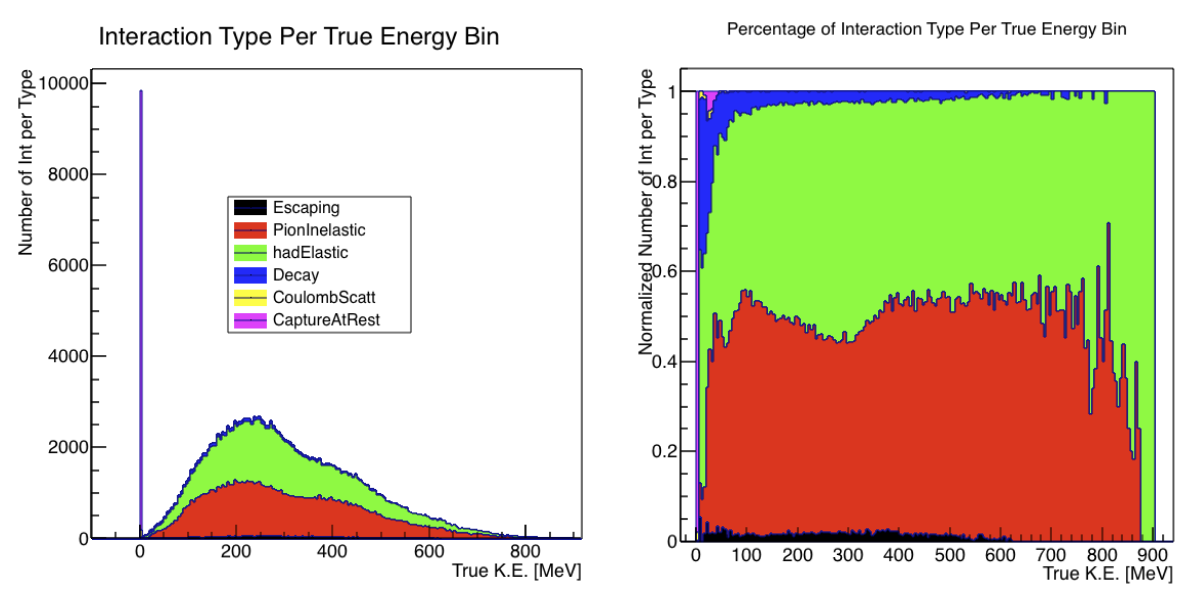
\includegraphics[scale=0.33]{./images/PiArIntTypesTrueFineBin.png}
\caption{(LHS): Number of $\pi^{-}$-Argon interaction types as a function of true kinetic energy bin. (RHS): Percentage of each $\pi^{-}$-Argon interaction type per bin. The top set of plots are binned in 50 MeV bins (similar to the analysis) while the bottom plots are binned more finely for illustration}
\label{fig:TrueInteractionTypes}
\end{figure}

Figure \ref{fig:TrueInteractionTypesRecoE} shows how this fact is exasperated when we take into account the smearing caused by using the reconstructed kinetic energy. This suggests that excluding the lowest energy bin (between 0~MeV$<$KE$<$50~MeV) may be a prudent move in order to avoid the capture-at-rest sample from contaminating the cross-section.

\begin{figure}[h!]
\centering
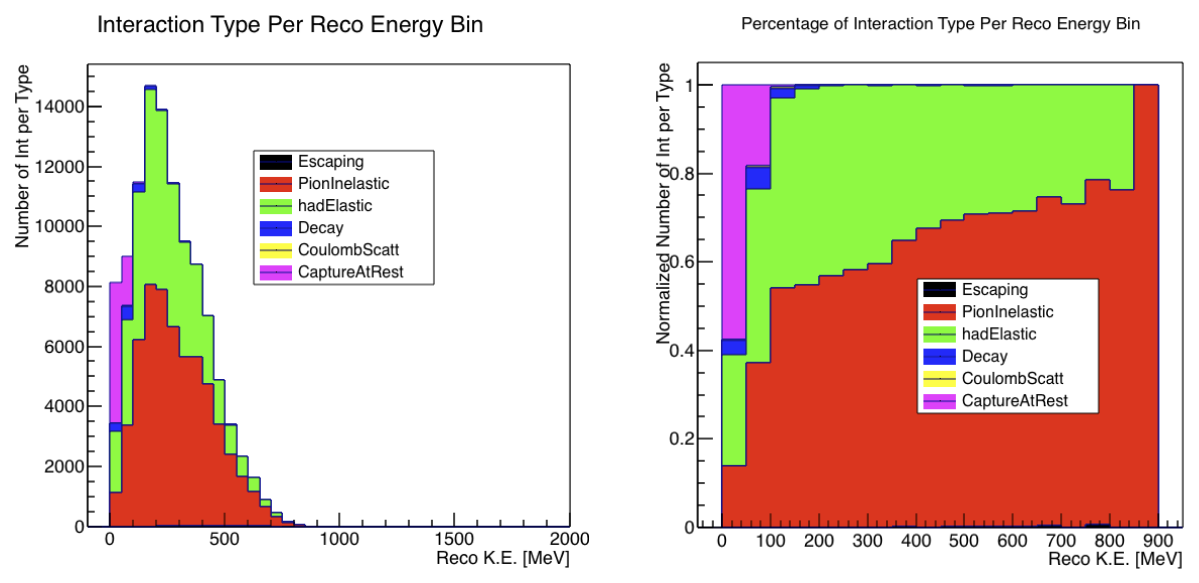
\includegraphics[scale=0.33]{./images/PiArIntTypesReco.png}
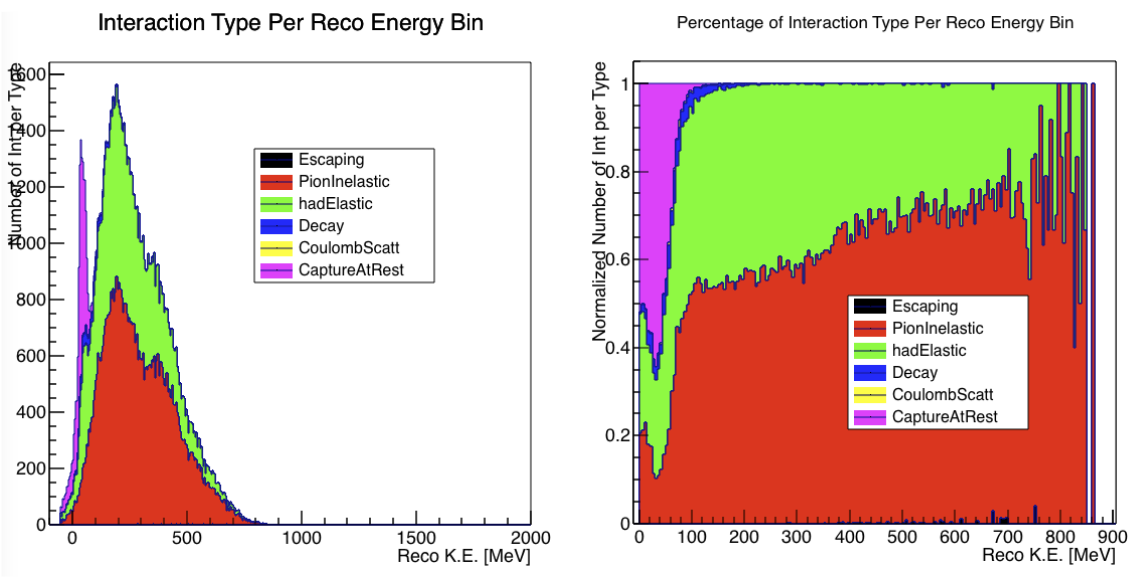
\includegraphics[scale=0.33]{./images/PiArIntTypesRecoFineBin.png}
\caption{(LHS): Number of $\pi^{-}$-Argon interaction types as a function of reconstructed kinetic energy bin. (RHS): Percentage of each $\pi^{-}$-Argon interaction type per bin. The top set of plots are binned in 50 MeV bins (similar to the analysis) while the bottom plots are binned more finely for illustration}
\label{fig:TrueInteractionTypesRecoE}
\end{figure}


%%%%%%%%%%%%%%%%%%%%%%%%%%%%%%%%%%%%%%%%%%%%%%%%%%%
\subsection{Validation Plots} \label{sec:ValidationPlots}
%%%%%%%%%%%%%%%%%%%%%%%%%%%%%%%%%%%%%%%%%%%%%%%%%%%
In this section we will cover a few different aspects of the validation of the data and Monte Carlo samples being used here. These checks include checks of the calorimetry, validation of the reconstruction by looking at a series of low level variables in both data and MC, and cross-checks of the thin-slice method.

%%%%%%%%%%%%%%%%%%%%%%%%%%%%%%%%%%%%%%%%%%%%%%%%%%%%%%%%%%%%
\subsubsection{Calorimetry Cross-check} \label{sec:calocrosscheck}
%%%%%%%%%%%%%%%%%%%%%%%%%%%%%%%%%%%%%%%%%%%%%%%%%%%%%%%%%%%%
\paragraph{\textbf{Wire-to-Wire Corrections}}

The wire response to charge has been observed to be non-uniform during Run-I and Run-II data taking. The pattern of the wire to wire variation stays fairly consistent across various runs and has been shown to be independent from the track inclination respect to the wire planes, track distance from the wire planes (i.e. from the drift time), track position along the wire and the cold electronics. More detail about these investigations can be found in \href{https://lartpc-docdb.fnal.gov:441/cgi-bin/ShowDocument?docid=1927}{docDB-1927}, with the best current hypothesis for the origin of this oscillation being the WRD cards that drove the 25' cables to the DAQ rack.


A correction factor is applied in order to restore the uniformity in the wire response to charge. The left hand side of Figure \ref{fig:wirebywire} shows the variation in the charge for each wire for a set of runs in Run-I. A mean correction factor for each wire is calculated and applied to the data to remove the effect of this non-uniform charge response. The right hand side of Figure \ref{fig:wirebywire} shows the effect of this correction on a sample of Run-I data, for the collection plane.

\begin{figure}[h!]
\centering
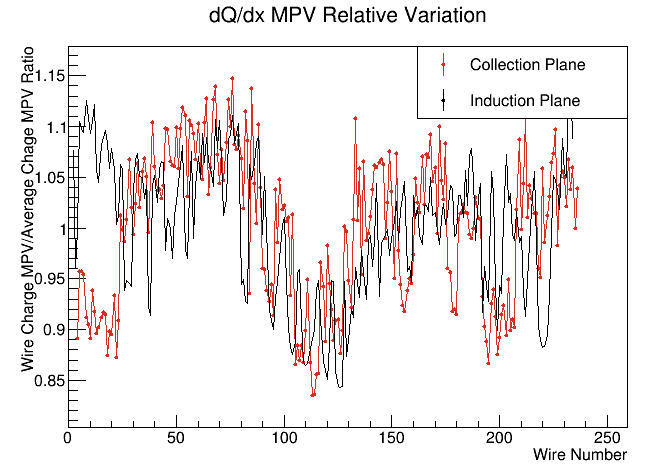
\includegraphics[scale=0.35]{./images/Run1WireCorrectionFactor.png}
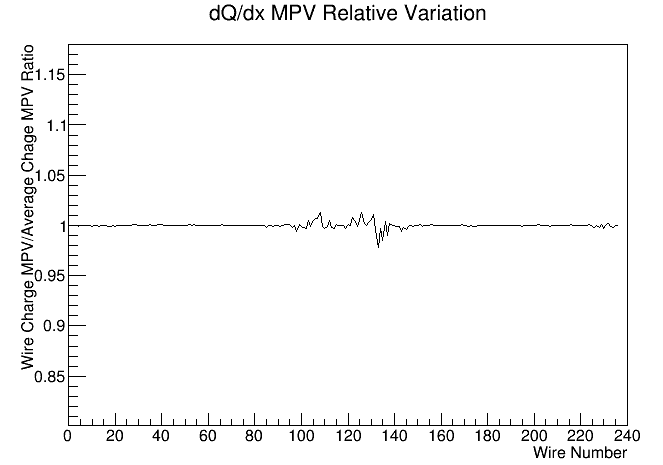
\includegraphics[scale=0.35]{./images/Run1WireCorrected.png}
\caption{(LHS): Deviation from the reference value of the $dQ/dx$ most probable value as calculated on each wire for a given plane. The reference value is obtained by averaging $dQ/dx$ over all the wires. Variations as high as 15\% are observed. Values for Induction (black) and Collection (red) planes are reported. (RHS): The corrected $dQ/dX$ response for Run-1 data sample, Collection plane only}
\label{fig:wirebywire}
\end{figure}

\paragraph{\textbf{Electron Lifetime Correction}}

The amount of charge per unit of length $dQ/dx$ collected at the wire plane is dependent on the distance traveled by the ionization charge in LAr because of quenching by the electronegative contaminants. In order to retrieve the original ionization charge, we need to correct for the attenuation factor, expressed in terms of electron lifetime and drift time. The full explanation of the method employed to measure the electron lifetime can be found in docDB-1804.

For Run-I and Run-II data, the electron lifetime is found using a sample of cosmic rays and stored in an online database. When the samples used in this analysis are reconstructed, they have a lifetime correction applied to account for the varying lifetime seen in LArIAT. The details of how this is applied in the calorimetry package is explained in \href{https://lartpc-docdb.fnal.gov:441/cgi-bin/ShowDocument?docid=1804}{docDB-1804}. Figure \ref{fig:LifetimeNOchargecorrection} shows an example of the lifetime derived for Run-I and Run-II data.

\begin{figure}[h!]
\centering
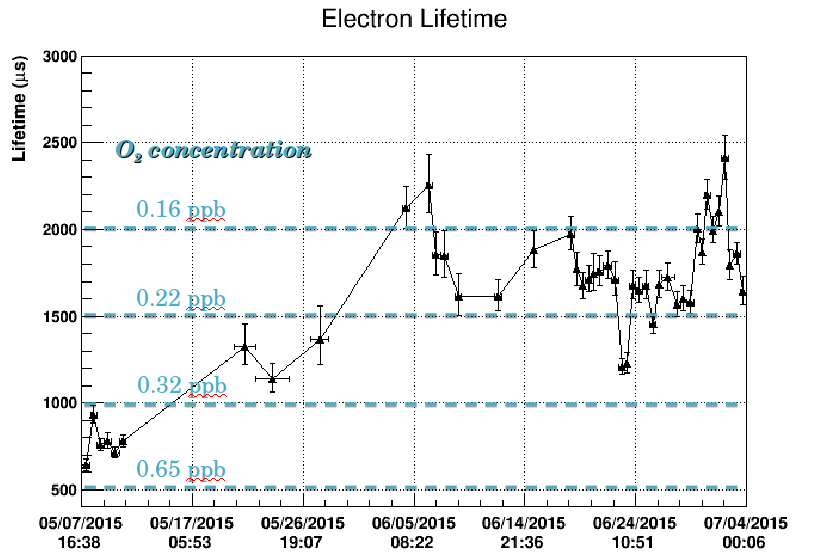
\includegraphics[scale=0.35]{./images/Run1Lifetime.png}
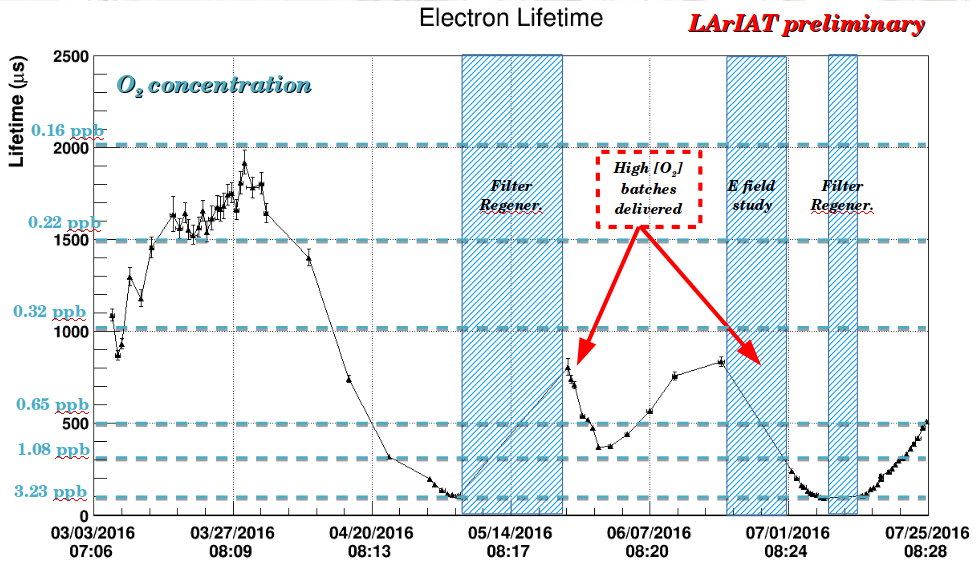
\includegraphics[scale=0.28]{./images/Run2Lifetime.png}
\caption{Electron lifetime for Run-I (Top) and Run-II (Bottom), obtained with the multi-track method (see DocDb 1804). Errors are statistical only.}
\label{fig:LifetimeNOchargecorrection}
\end{figure}

\paragraph{\textbf{Calorimetry Constant Tuning}}
The calorimetry constants used in this data analysis were determined from a sample of data and Monte Carlo spanning Run I and Run II. The calibration method, described in greater detail in \href{https://lartpc-docdb.fnal.gov:441/cgi-bin/ShowDocument?docid=2513}{docDB-2513}, is predicated on the Bethe-Bloch description of the mean rate of energy loss for various particle species. The basic idea of this calibration technique is to utilize a portion of a track within the LArTPC that has a well known momentum and particle species to measure the energy deposited per unit length (dE/dX) as recorded inside the TPC. Once a sample of particles dE/dX has been measured at various momentums, we then tune to calorimetry constants within the reconstruction software to align these measured values to match the theoretical ones.

Figure \ref{fig:dEdXvsMomentum} shows the calorimetry response for the $\pi, \mu, e$-High-Yield data sample used in this analysis. The selection method for this sample is to take each  track within the TPC that is uniquely matched to a wire-chamber track and use the measured momentum for that track. We require the track to be of a minimum length of 10~cm long (to ensure we are away from any interaction point where the track may be broken into subsequent tracks). We then take the first twelve spacepoints of the track (excluding the first point to avoid edge effects near the field cage) and sample the reconstructed dE/dX for each point along the track. On average, this samples 5~cm of the track and takes the dE/dX measurements are then put into a histogram that corresponds to measured momentum of the track.

\begin{figure}[h!]
\centering
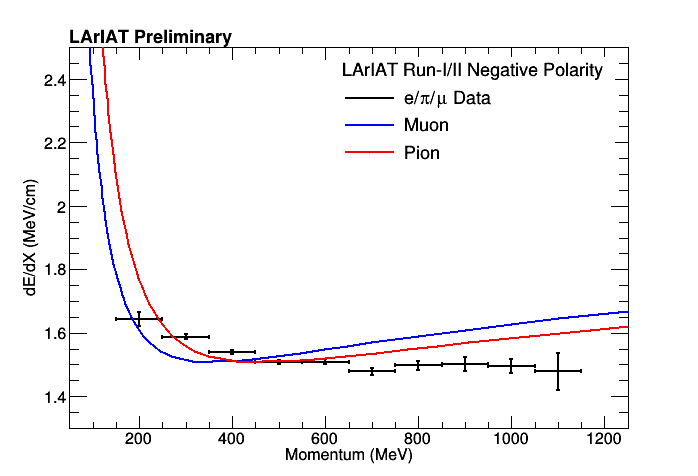
\includegraphics[scale=0.33]{./images/dEdXvsMomentumCombined.png}
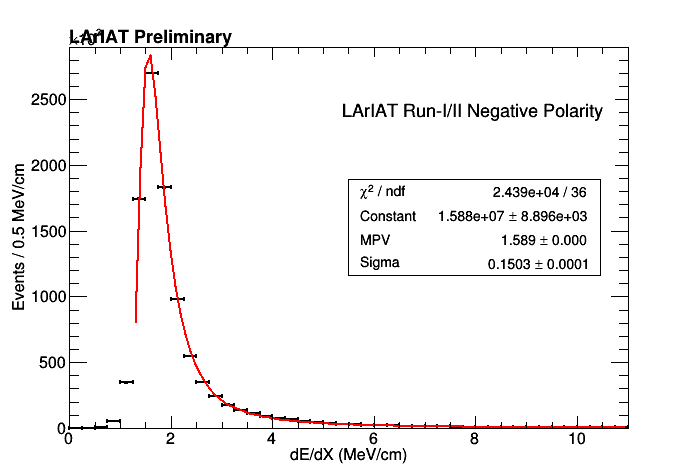
\includegraphics[scale=0.33]{./images/dEdXDataFit.png}
\caption{(LHS)dE/dX most probable value (MPV) as a function of momentum for the sample of events used in this analysis. (RHS) dE/dX for the sample used in this analysis fit with a Landau between 1.25 MeV/cm $<$ dE/dX $<$ 12 MeV/cm (similarly to what was done in the calibration procedure), returning a MPV of 1.589 MeV/cm. These values are obtained using the calorimetry constants derived in \href{https://lartpc-docdb.fnal.gov:441/cgi-bin/ShowDocument?docid=2513}{docDB-2513}}
\label{fig:dEdXvsMomentum}
\end{figure}

\newpage
%%%%%%%%%%%%%%%%%%%%%%%%%%%%%%%%%%%%%%%%%%%%%%%%%%%%%%%%%%%%
\subsubsection{Data/MC Comparisons} \label{sec:DataMCCompare}
%%%%%%%%%%%%%%%%%%%%%%%%%%%%%%%%%%%%%%%%%%%%%%%%%%%%%%%%%%%%

Here we present a series of low-level plots which validate the data and Monte Carlo reconstruction. Each set of plots is shown with the y-axis in both linear and log scale to allow for comparisons in the bulk as well as the tale. Commentary on any set of plots is made in the caption.

\begin{figure}[h!]
\centering
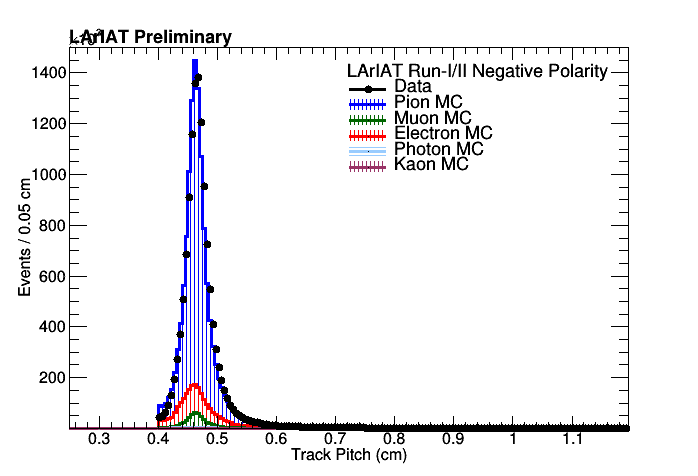
\includegraphics[scale=0.33]{./images/TrackPitch.png}
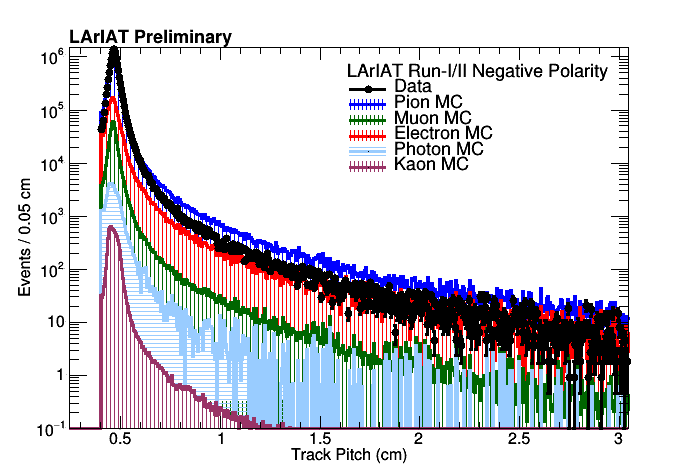
\includegraphics[scale=0.33]{./images/TrackPitchLog.png}
\caption{The reconstructed track pitch for data and Monte Carlo. Monte Carlo is scaled to data in the proportions which represent both the expected beam composition (Table \ref{tab:beamcomp1}) and the selection efficiency for that sample (Table \ref{tab:MCPercentageTable}. The data and MC agree well in the bulk of the sample, with the high end of the track pitch tail showing some disagreement, suggesting different pathologies in the data and MC cause points to be skipped along the track. These difference are quantitatively small and thus shouldn't impact the final result. }
\label{fig:DataMCTrackPitch}
\end{figure}

\begin{figure}[h!]
\centering
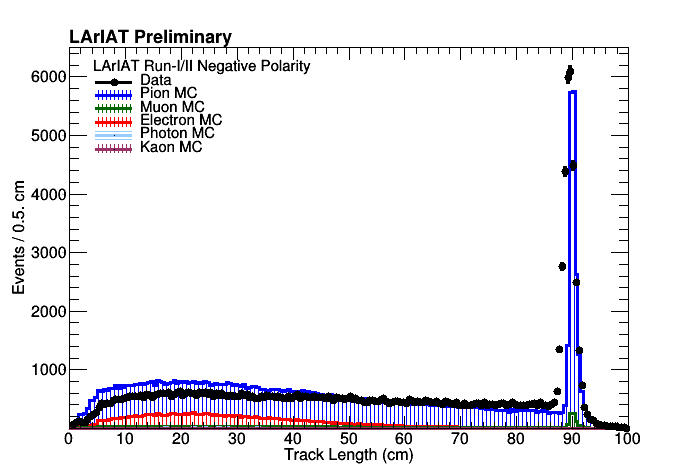
\includegraphics[scale=0.33]{./images/TrackLength.png}
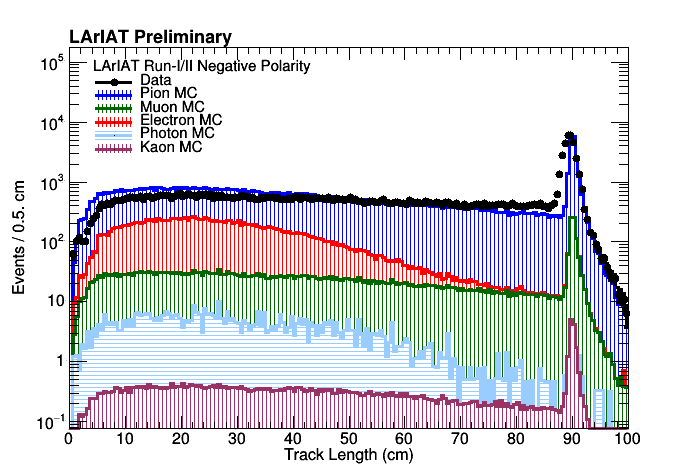
\includegraphics[scale=0.33]{./images/TrackLengthLog.png}
\caption{The reconstructed track length for data and Monte Carlo. Monte Carlo is scaled to data in the proportions which represent both the expected beam composition (Table \ref{tab:beamcomp1}) and the selection efficiency for that sample (Table \ref{tab:MCPercentageTable}. The data and MC agree overall with the MC slightly over-predicting the shortest tracks where the electron and photon samples dominate. Later plots show these slight difference to be negligible to the overall analysis.}
\label{fig:DataMCTrackLength}
\end{figure}

\begin{figure}[h!]
\centering
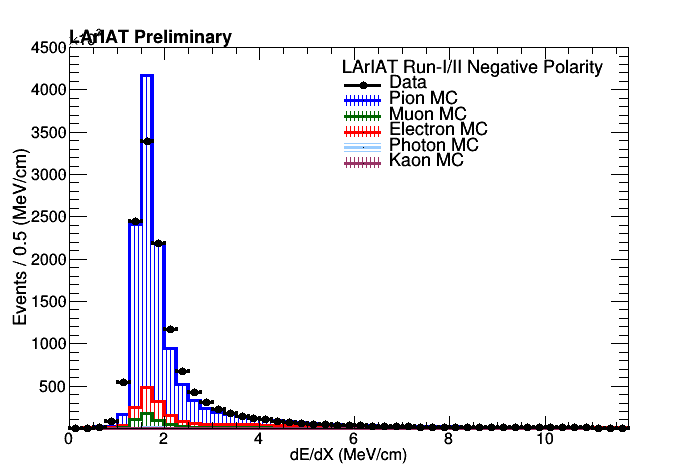
\includegraphics[scale=0.33]{./images/dEdX.png}
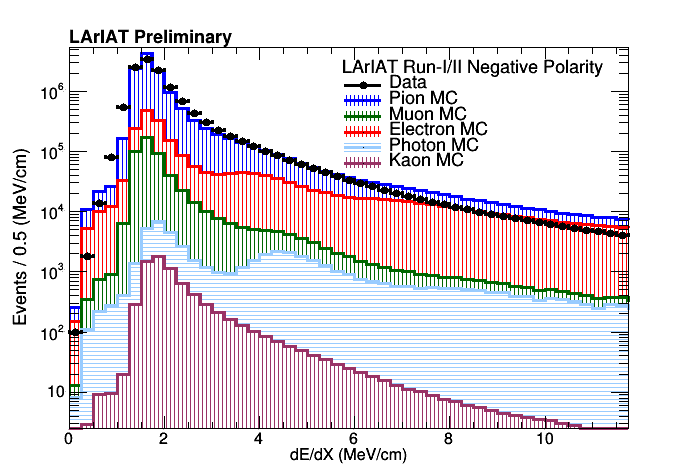
\includegraphics[scale=0.33]{./images/dEdXLog.png}
\caption{The reconstructed energy deposited per unit length (dE/dX) for data and Monte Carlo. Monte Carlo is scaled to data in the proportions which represent both the expected beam composition (Table \ref{tab:beamcomp1}) and the selection efficiency for that sample (Table \ref{tab:MCPercentageTable}. The data and MC agree in the most probable value (MPV) and in the shape. There is a slight difference in the highest side tail for the dE/dX $>$ 6 MeV/cm. This corresponds to a very small overall component of the sample and thus should only cause a slight difference in the computation of the kinetic energy for the track.}
\label{fig:DataMCdEdX}
\end{figure}

\begin{figure}[h!]
\centering
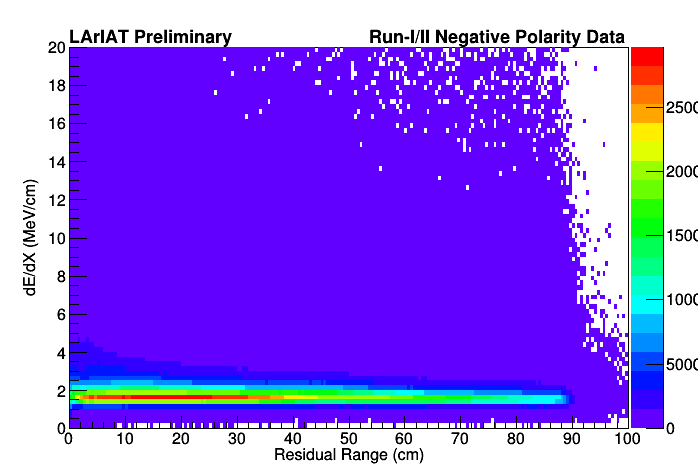
\includegraphics[scale=0.33]{./images/dEdXvsRRData.png}
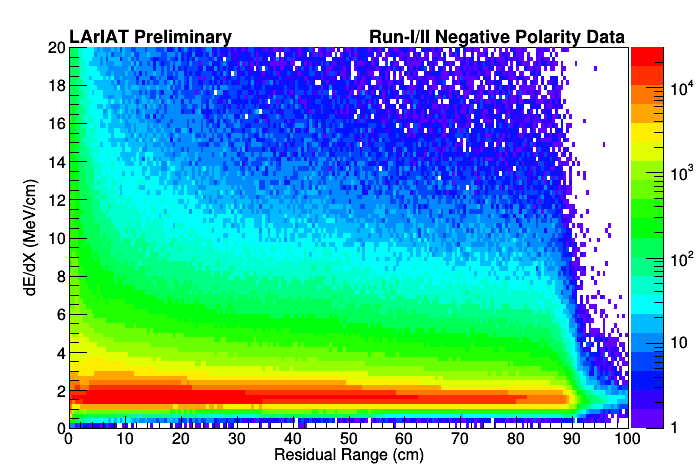
\includegraphics[scale=0.33]{./images/dEdXvsRRDataLog.png}
\caption{The reconstructed energy deposited per unit length (dE/dX) versus the Residual  Range for the data sample selected in Table \ref{tab:CutSummary}. These results agree well with Figure \ref{fig:PionMCdEdXvsRR} giving confidence that the sample of data is dominated by minimum ionizing particles (such as pions) and that the samples are well calibrated.}
\label{fig:DatadEdXvsRR}
\end{figure}

\begin{figure}[h!]
\centering
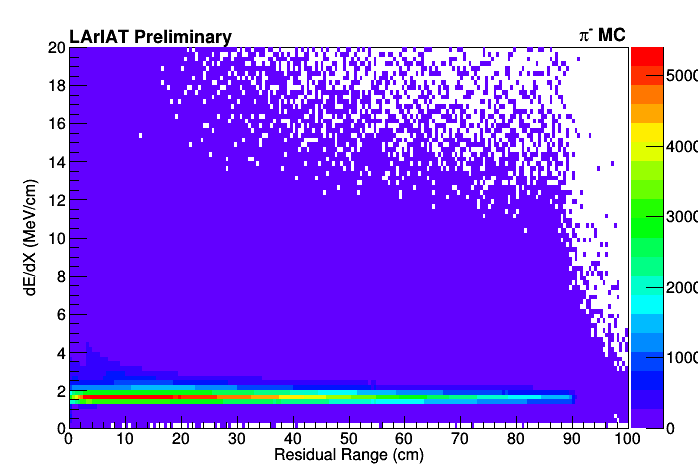
\includegraphics[scale=0.33]{./images/dEdXvsRRPionMC.png}
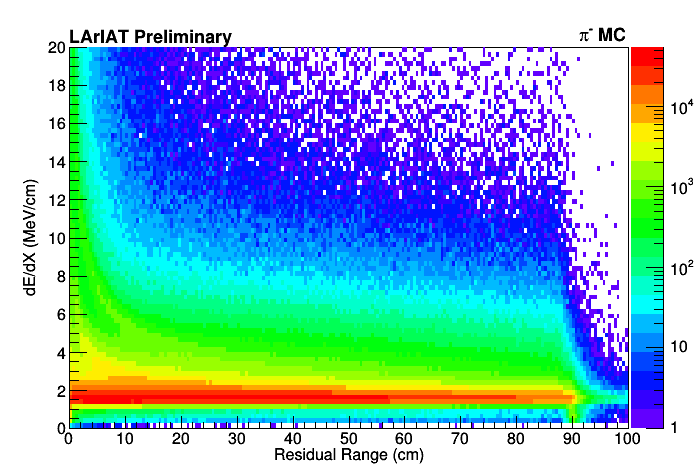
\includegraphics[scale=0.33]{./images/dEdXvsRRPionMCLog.png}
\caption{The reconstructed energy deposited per unit length (dE/dX) versus the Residual  Range for the Pion MC sample selected in Table \ref{tab:MCRunIICutSummary}.}
\label{fig:PionMCdEdXvsRR}
\end{figure}

\newpage
%%%%%%%%%%%%%%%%%%%%%%%%%%%%%%%%%%%%%%%%%%%%%%%%%%%%%%%%%%%%
\subsubsection{Energy Reconstruction Cross-Check} \label{sec:ERecoCrossCheck}
%%%%%%%%%%%%%%%%%%%%%%%%%%%%%%%%%%%%%%%%%%%%%%%%%%%%%%%%%%%%

Figure \ref{fig:RecoEvsTrueE} shows the reconstructed kinetic energy at the interaction point for a sample of $\pi^{-}$ MC compared to the true energy the pion had at the interaction point. The reconstructed energy at the interaction point is calculated by
\begin{equation}
KE_{Interaction} = \sqrt{P_{WCtrk}^2 + m_{\pi}^2} - E_{Loss} - (\Sigma dE/dX_{i} \times Pitch)
\end{equation}
where $P_{WCtrk}$ represents the momentum as simulated by the equivalent of the wire-chamber track in the MC, $m_{\pi}$ is the mass of the pion, $E_{Loss}$ is the flat energy correction which takes into account the energy loss due to the interviening material between WC-4 and the front face of the TPC (here assumed to be 40 MeV) and $\Sigma dE/dX_{i} \times Pitch$ is the energy loss using the reconstructed track. This shows very good agreement with a linear regression fit which returns a near diagonal line with a y-intercept close to zero.

\begin{figure}[htb]
\centering
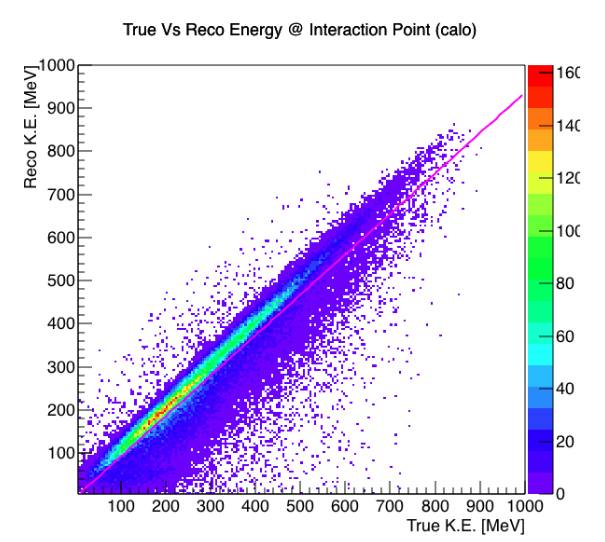
\includegraphics[scale=0.38]{./images/RecoEvsTrueE.png}
\caption{Reconstructed kinetic energy at the interaction point for a sample of DDMC $\pi^{-}$ compared to the kinetic energy of the pion as calculated from Geant4. The plot is fit with a linear regression which returns an R$^{2}$ = 0.87 and a y intercept of -1.72 MeV with a slope of 0.94.}
\label{fig:RecoEvsTrueE}
\end{figure}

As a point of comparison, Figure \ref{fig:LengthRecoEvsTrueE} shows the reconstructed kinetic energy at the interaction point versus the true energy at the interaction point where instead of using the calorimetry tools we calculate the reconstructed energy using the length of the track. Here the reconstructed energy is given by 
\begin{equation}
KE_{Interaction} = \sqrt{P_{WCtrk}^2 + m_{\pi}^2} - E_{Loss} - (2.1 MeV/cm \times Length_{Reco})
\end{equation}
where 2.1 MeV/cm is the mean of the dE/dX distribution and $Length_{Reco}$ is the reconstructed length of the track up to its interaction point. This also gives good agreement with only a slight improvement on the linear regression fit as compared to the sample using the reconstructed calorimetry.
 
\begin{figure}[htb]
\centering
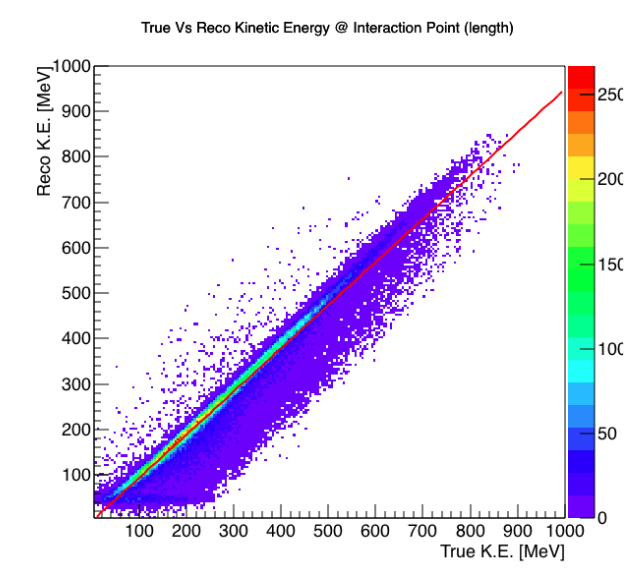
\includegraphics[scale=0.38]{./images/LengthRecoEvsTrueE.png}
\caption{Length based reconstructed kinetic energy at the interaction point for a sample of DDMC $\pi^{-}$ compared to the kinetic energy of the pion as calculated from Geant4. The plot is fit with a linear regression which returns an R$^{2}$ = 0.92 and a y intercept of -1.26 MeV with a slope of 0.95.}
\label{fig:LengthRecoEvsTrueE}
\end{figure}

For completeness, the calorimetry based method is compared to the length based method in Figure \ref{fig:CaloMethvsLengthMeth}. The two methods return very nearly to same answer over the range of kinetic energy seen in LArIAT. This gives us confidence in continuing to use the calorimetry based reconstruction of our kinetic energy as the method for calculating the cross-section as a function of kinetic energy.

\begin{figure}[htb]
\centering
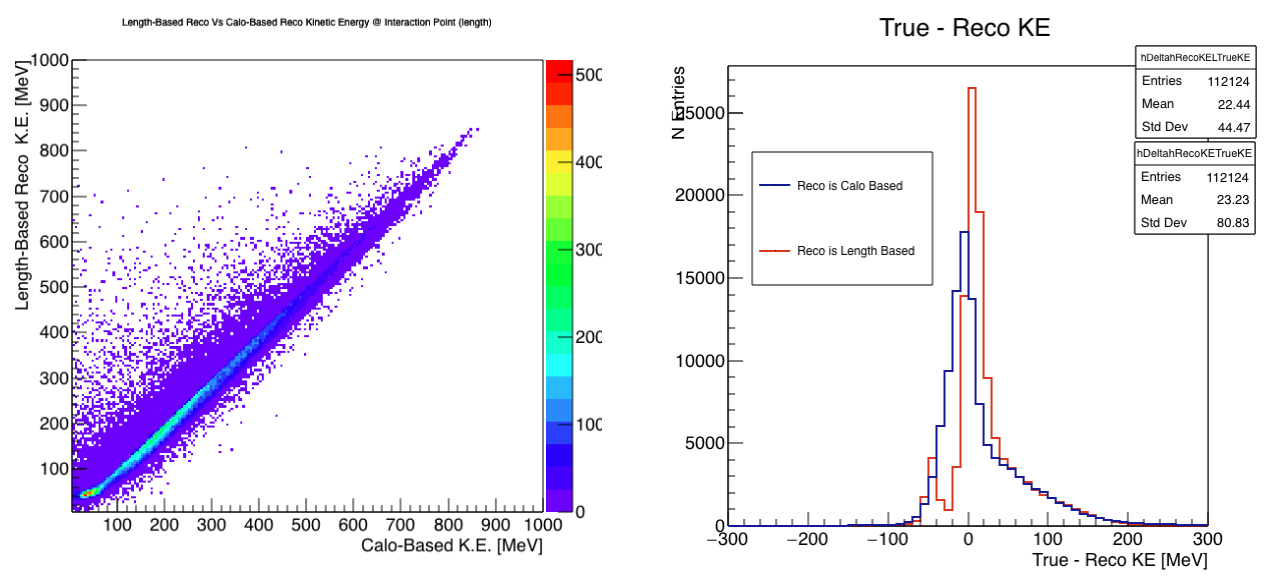
\includegraphics[scale=0.38]{./images/CaloMethodsCompared.png}
\caption{(LHS) Length based kinetic energy versus the calorimetry based kinetic energy. (RHS) Calculated the $\Delta$E (True - Reco) for the two methods. Red: Length Based, Blue: Calorimetry Based. }
\label{fig:CaloMethvsLengthMeth}
\end{figure}



\newpage
\newpage
\section{Results}\label{sec:Results}
In this section we overview the results of the event selection outlined in the previous sections. Section \ref{sec:DataReduction} gives the breakdown of data events passing all our selection cuts and presents the beamline plots for this sample. Section \ref{sec:MCReduction} provides the similar breakdown of the MC events passing the selection cuts. Section \ref{sec:ValidationPlots} overviews a series of Data/MC comparisons to validate that the sample of simulated events is well reproduced in the data. Finally, Section \ref{sec:CrossSection} shows the inclusive $\pi^{-}$-Argon cross-section.


%%%%%%%%%%%%%%%%%%%%%%%%%%%%%%%%%%%%%%%%%%%%%%%%%%%
\subsection{Data Event Reduction} \label{sec:DataReduction}
%%%%%%%%%%%%%%%%%%%%%%%%%%%%%%%%%%%%%%%%%%%%%%%%%%%
Table \ref{tab:CutSummary} gives the event reduction for the negative polarity $\pi, \mu, e$ data sample for Run-I, Run-II, and combined. The definition of the cuts presented here are given in Section \ref{sec:TPCCandidateSelect}

%%% Put event reduction tables here 
\begin{table}[htb]
	\begin{center}
	\resizebox{0.95\textwidth}{!}{%
	\begin{tabular}{|c|c|c|c|}
	\hline
	%\multicolumn{5}{|c|}{\textbf{Summary of inclusive NC $\pi^{0}$ Event Selection Cuts}} \\
	%\hline \hline
	  \textbf{Event Selection} & Run-I Negative Polarity & Run-II Negative Polarity & Combined  \\
	\hline
	Total Number of Beam Events & 113,336 & 1,585,598 & 1,698,934 \\
	\hline
	$\pi, \mu, e$ Mass Selection & 20,653 & 493,455 & 514,108 \\
	\hline
	20~ns $<$TOF$<$27 & 20,577 & 485,159 & 505,736 \\
	\hline
	Requiring an upstream TPC Track within $z<2$cm & 18,882  & 403,561   &  422,443 \\
	\hline
	$<4$ tracks in the first $z<14$cm & 12,910  & 316,451  & 329,361 \\
	\hline
	Electromagnetic shower rejection & 9,824  & 232,510  &  242,334 \\
	\hline
	Unique match between WC/TPC Track & 5,500 & 120,956 & 126,456\\
	\hline
	\hline
	\end{tabular}}
	\caption{Summary of the events passing the inclusive pion selection criteria.} \label{tab:CutSummary}
	\end{center}
\end{table}

For the combined Run-I/Run-II sample Figures \ref{fig:WCandTOFBeamlinePlot}, \ref{fig:DeltaXDeltaY} show the time-of-flight and momentum spectrum as well as the results of the WC/TPC matching. The addition of a cut on the TOF to require  20~ns $<$TOF$<$27 is to clean up the low momentum high TOF events seen in Figure \ref{fig:WCandTOFBeamlinePlot}.

\begin{figure}[h!]
\centering
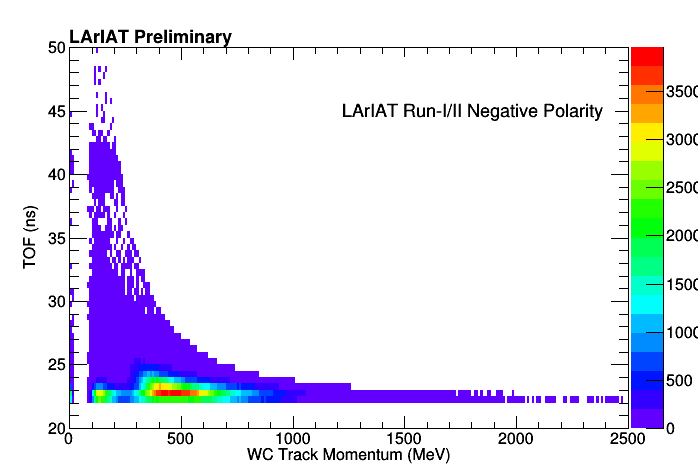
\includegraphics[scale=0.30]{./images/TOFvsWCTrk.png}
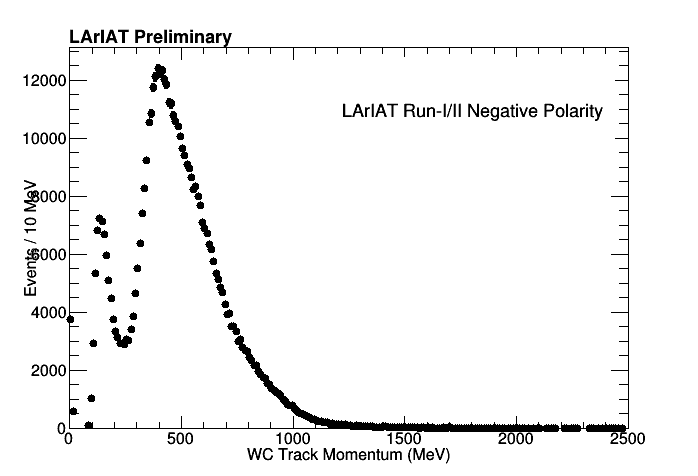
\includegraphics[scale=0.30]{./images/wctrkMomentum.png}
\caption{(Left) Time-of-Flight vs Wire Chamber Track Momentum. (Right) The momentum spectrum for our sample.}
\label{fig:WCandTOFBeamlinePlot}
\end{figure}

\begin{figure}[h!]
\centering
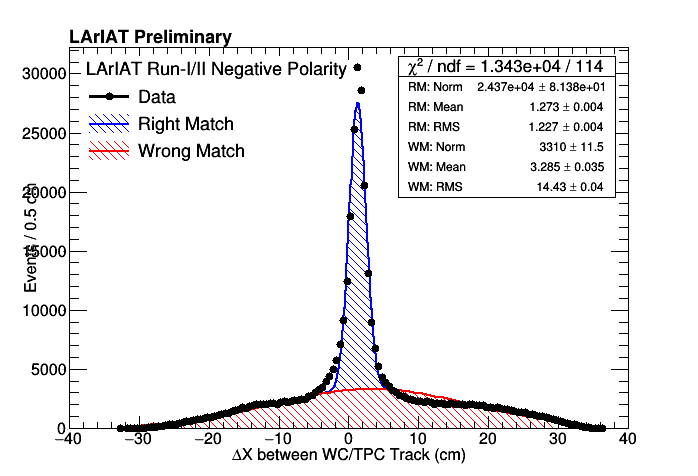
\includegraphics[scale=0.30]{./images/DeltaX.png}
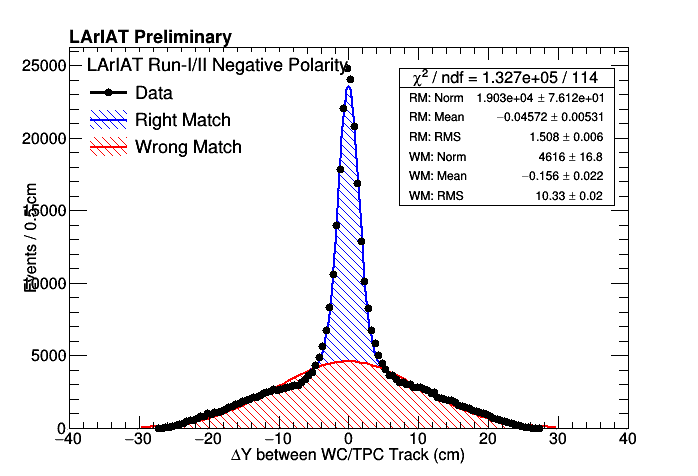
\includegraphics[scale=0.30]{./images/DeltaY.png}
\caption{The $\Delta X$ and $\Delta Y$ distributions prior to requiring the match between the TPC and WC track.}
\label{fig:DeltaXDeltaY}
\end{figure}

%%%%%%%%%%%%%%%%%%%%%%%%%%%%%%%%%%%%%%%%%%%%%%%%%%%
\subsection{MC Event Reduction} \label{sec:MCReduction}
%%%%%%%%%%%%%%%%%%%%%%%%%%%%%%%%%%%%%%%%%%%%%%%%%%%
Table \ref{tab:MCRunIICutSummary} shows a similar event reduction as was done in previous section for the sample of Run-II MC.

%%% Put event reduction tables here 
\begin{table}[htb]
	\begin{center}
	\resizebox{0.98\textwidth}{!}{%
	\begin{tabular}{|c|c|c|c|c|c|}
	\hline
	%\multicolumn{5}{|c|}{\textbf{Summary of inclusive NC $\pi^{0}$ Event Selection Cuts}} \\
	%\hline \hline
	  \textbf{Event Selection} & Run-II High Yield & Run-II High Yield & Run-II High Yield & Run-II High Yield & Run-II High Yield \\
	   & $\pi^{-}$ MC & $\mu^{-}$ MC  & $e^{-}$ MC & $K^{-}$ MC & $\gamma$ MC \\
	\hline
	Total Number of MC Events & 359,000 & 361,000 & 361,000 & 185,000 & 193,500 \\
	\hline
	MC-Particle Reaches the TPC & 245,511 & 246,874 & 323,997 & 95,391 & 72,782 \\
	\hline
	Requiring an upstream TPC Track within $z<2$cm & 220,752 & 221,966 & 254,218 & 82,407 & 5,782 \\
	\hline
	$<4$ tracks in the first $z<14$cm & 220,454 & 221,666 & 239,406 & 81,369 & 5,730 \\
	\hline
	Electromagnetic shower rejection & 218,068 & 219,274 & 94,293 & 77,281 & 2,471 \\
	\hline
	Unique match between WC/TPC Track & 180,341 & 181,327 & 46,133 & 67,420 & 1,670\\
	\hline
	\hline
	\end{tabular}}
	\caption{Summary of the MC events passing the inclusive pion selection criteria.} \label{tab:MCRunIICutSummary}
	\end{center}
\end{table}

Since the data has significantly more statistics for Run-II compared to Run-I ($\sim$22:1 ratio), the Run-II MC is used for the purposes of comparison as mixing of the two samples in this ratio does not change the final result. For the sake of completeness, Table \ref{tab:MCRunICutSummary} shows a similar event reduction as was done in previous section for the sample of Run-I MC.

%%% Put event reduction tables here 
\begin{table}[htb]
	\begin{center}
	\resizebox{0.95\textwidth}{!}{%
	\begin{tabular}{|c|c|c|c|c|c|}
	\hline
	%\multicolumn{5}{|c|}{\textbf{Summary of inclusive NC $\pi^{0}$ Event Selection Cuts}} \\
	%\hline \hline
	  \textbf{Event Selection} & Run-I High Yield & Run-I High Yield & Run-I High Yield & Run-I High Yield & Run-I High Yield \\
	   & $\pi^{-}$ MC & $\mu^{-}$ MC  & $e^{-}$ MC & $K^{-}$ MC & $\gamma$ MC \\
	\hline
	Total Number of MC Events & 357,000 &  &  & & 193,500 \\
	\hline
	MC-Particle Reaches the TPC & 258,294 &  &  & & 72,782 \\
	\hline
	Requiring an upstream TPC Track within $z<2$cm & 233,763  &  &  & & 5,782 \\
	\hline
	$<4$ tracks in the first $z<14$cm & 233,447  &  &  & & 5,730 \\ 
	\hline
	Electromagnetic shower rejection & 230,960  &  & & & 2,471 \\
	\hline
	Unique match between WC/TPC Track & 189,670 &  & & & 1,670\\
	\hline
	\hline
	\end{tabular}}
	\caption{Summary of the MC events passing the inclusive pion selection criteria.} \label{tab:MCRunICutSummary}
	\end{center}
\end{table}

Table \ref{tab:MCPercentageTable} summarizes the fraction of events passing all the inclusive pion analysis cuts. This fraction is calculated using the number of events passing all the cuts divided by the number of MC events which reach the front face of the TPC. We use the number of MC events reaching the front face of the TPC instead of the total number of MC events because using the latter would mis-represent the efficiency of the TPC based cuts.

\begin{table}[h!]
\centering
\resizebox{0.95\textwidth}{!}{%
\begin{tabular}{|c|c|c|c|c|c|}
\hline
 & $\pi^{-}$ MC & $\mu^{-}$ MC  & $e^{-}$ MC & $K^{-}$ MC & $\gamma$ MC \\
\hline
\textbf{Percent of events passing cut} & 73.5$\%$ & 73.4$\%$ & 14.2 $\%$ & 70.6$\%$ & 2.3$\%$ \\
\hline
\end{tabular}}
\caption{Fraction of MC Events passing inclusive pion analysis cuts.}
\label{tab:MCPercentageTable}
\end{table}

It should also be noted that the efficiency for selecting $K^{-}$ events is likely to be overly inflated here both because they make up a very small percentage of the negative polarity beam $< 1\%$ and because these cuts do not take into account the beamline mass filter applied to the data.

Figure \ref{fig:TrueInteractionTypes} shows the breakdown of $\pi^{-}$-Argon interaction types as a function of true kinetic energy taken from the pion DDMC. One important feature of this plot to note that pion capture-at-rest dominates. This process is not one which should be included in the total $\pi^{-}$-Argon interaction cross-section.

\begin{figure}[h!]
\centering
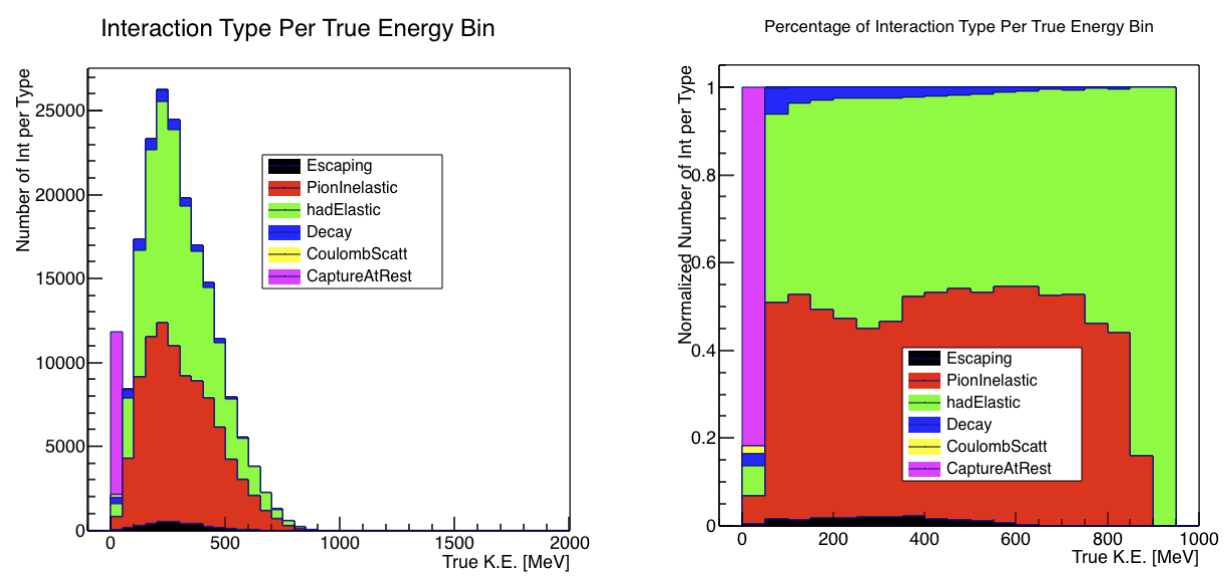
\includegraphics[scale=0.33]{./images/PiArIntTypesTrue.png}
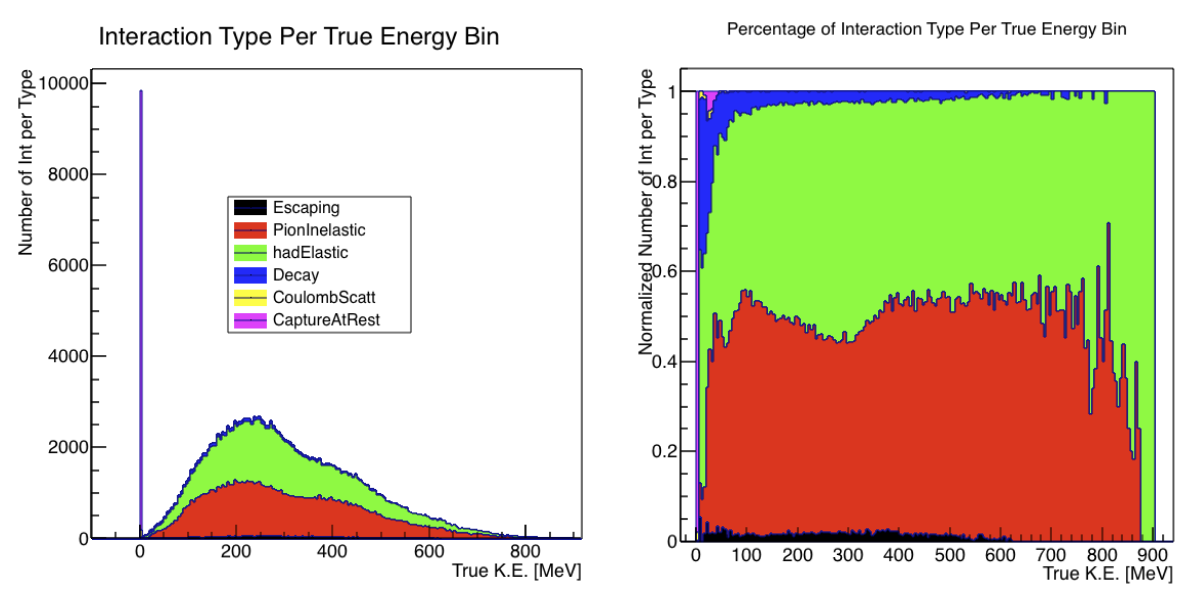
\includegraphics[scale=0.33]{./images/PiArIntTypesTrueFineBin.png}
\caption{(LHS): Number of $\pi^{-}$-Argon interaction types as a function of true kinetic energy bin. (RHS): Percentage of each $\pi^{-}$-Argon interaction type per bin. The top set of plots are binned in 50 MeV bins (similar to the analysis) while the bottom plots are binned more finely for illustration}
\label{fig:TrueInteractionTypes}
\end{figure}

Figure \ref{fig:TrueInteractionTypesRecoE} shows how this fact is exasperated when we take into account the smearing caused by using the reconstructed kinetic energy. This suggests that excluding the lowest energy bin (between 0~MeV$<$KE$<$50~MeV) may be a prudent move in order to avoid the capture-at-rest sample from contaminating the cross-section.

\begin{figure}[h!]
\centering
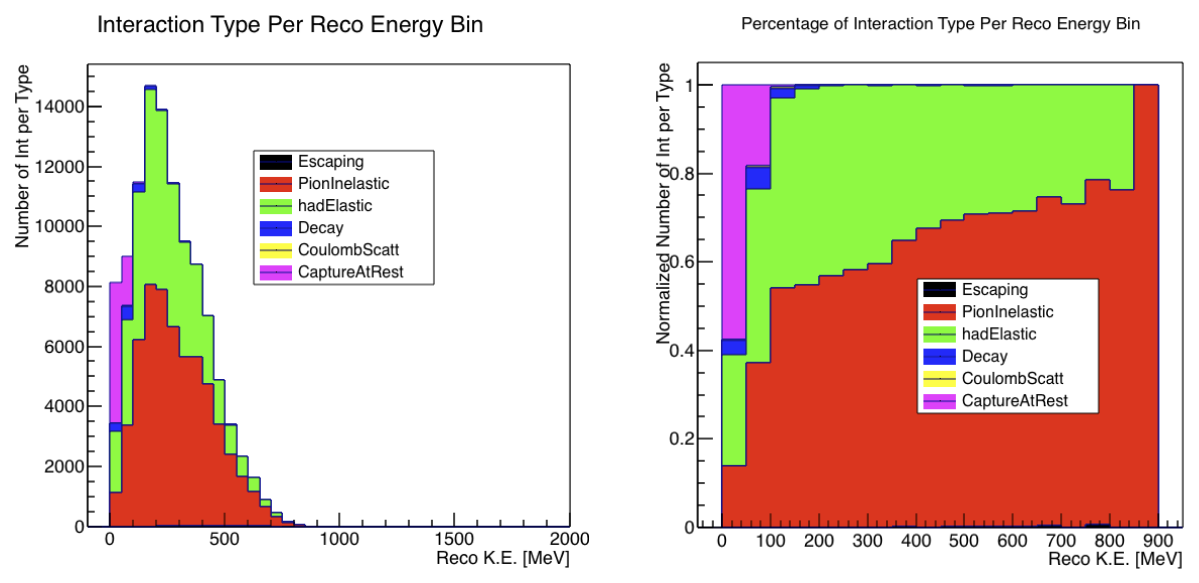
\includegraphics[scale=0.33]{./images/PiArIntTypesReco.png}
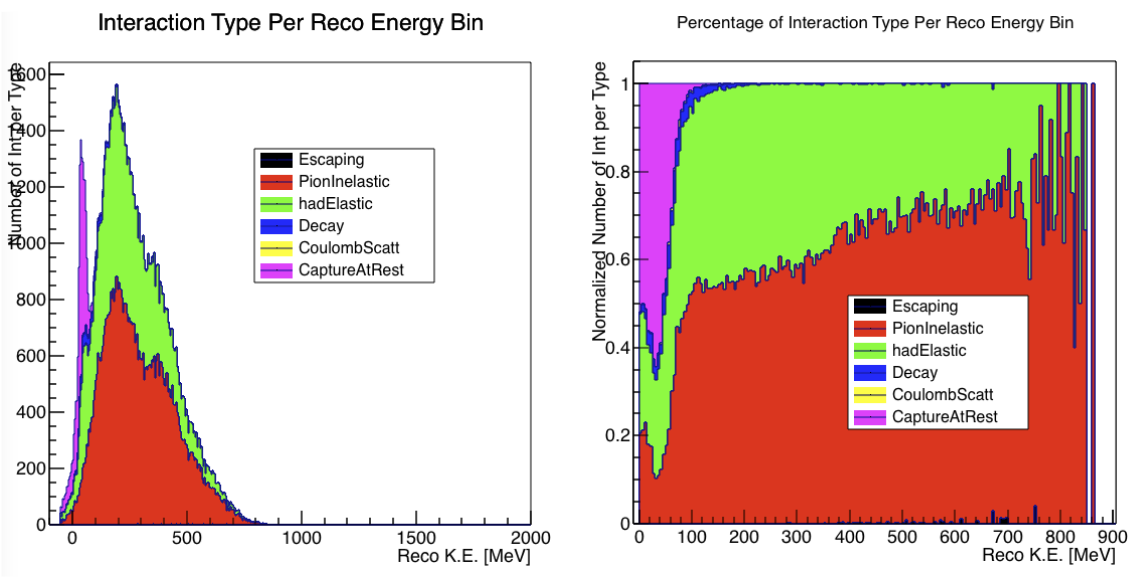
\includegraphics[scale=0.33]{./images/PiArIntTypesRecoFineBin.png}
\caption{(LHS): Number of $\pi^{-}$-Argon interaction types as a function of reconstructed kinetic energy bin. (RHS): Percentage of each $\pi^{-}$-Argon interaction type per bin. The top set of plots are binned in 50 MeV bins (similar to the analysis) while the bottom plots are binned more finely for illustration}
\label{fig:TrueInteractionTypesRecoE}
\end{figure}


%%%%%%%%%%%%%%%%%%%%%%%%%%%%%%%%%%%%%%%%%%%%%%%%%%%
\subsection{Validation Plots} \label{sec:ValidationPlots}
%%%%%%%%%%%%%%%%%%%%%%%%%%%%%%%%%%%%%%%%%%%%%%%%%%%
In this section we will cover a few different aspects of the validation of the data and Monte Carlo samples being used here. These checks include checks of the calorimetry, validation of the reconstruction by looking at a series of low level variables in both data and MC, and cross-checks of the thin-slice method.

%%%%%%%%%%%%%%%%%%%%%%%%%%%%%%%%%%%%%%%%%%%%%%%%%%%%%%%%%%%%
\subsubsection{Calorimetry Cross-check} \label{sec:calocrosscheck}
%%%%%%%%%%%%%%%%%%%%%%%%%%%%%%%%%%%%%%%%%%%%%%%%%%%%%%%%%%%%
\paragraph{\textbf{Wire-to-Wire Corrections}}

The wire response to charge has been observed to be non-uniform during Run-I and Run-II data taking. The pattern of the wire to wire variation stays fairly consistent across various runs and has been shown to be independent from the track inclination respect to the wire planes, track distance from the wire planes (i.e. from the drift time), track position along the wire and the cold electronics. More detail about these investigations can be found in \href{https://lartpc-docdb.fnal.gov:441/cgi-bin/ShowDocument?docid=1927}{docDB-1927}, with the best current hypothesis for the origin of this oscillation being the WRD cards that drove the 25' cables to the DAQ rack.


A correction factor is applied in order to restore the uniformity in the wire response to charge. The left hand side of Figure \ref{fig:wirebywire} shows the variation in the charge for each wire for a set of runs in Run-I. A mean correction factor for each wire is calculated and applied to the data to remove the effect of this non-uniform charge response. The right hand side of Figure \ref{fig:wirebywire} shows the effect of this correction on a sample of Run-I data, for the collection plane.

\begin{figure}[h!]
\centering
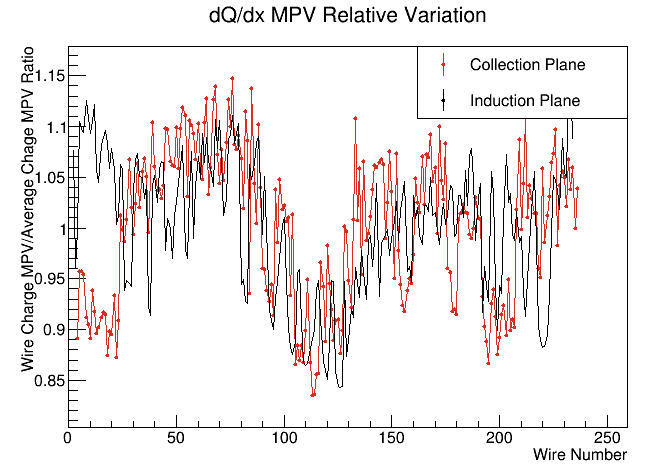
\includegraphics[scale=0.35]{./images/Run1WireCorrectionFactor.png}
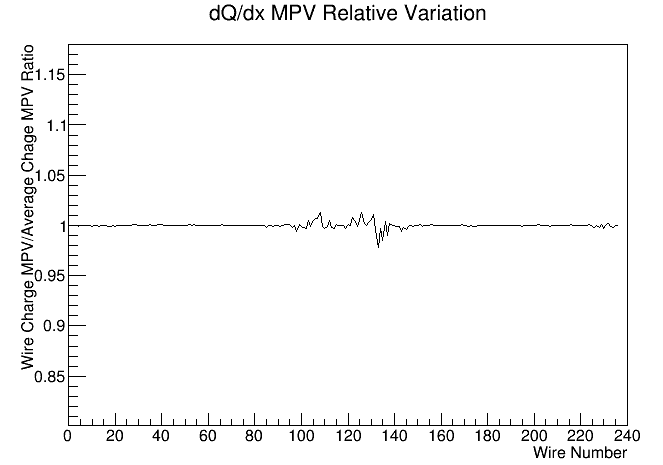
\includegraphics[scale=0.35]{./images/Run1WireCorrected.png}
\caption{(LHS): Deviation from the reference value of the $dQ/dx$ most probable value as calculated on each wire for a given plane. The reference value is obtained by averaging $dQ/dx$ over all the wires. Variations as high as 15\% are observed. Values for Induction (black) and Collection (red) planes are reported. (RHS): The corrected $dQ/dX$ response for Run-1 data sample, Collection plane only}
\label{fig:wirebywire}
\end{figure}

\paragraph{\textbf{Electron Lifetime Correction}}

The amount of charge per unit of length $dQ/dx$ collected at the wire plane is dependent on the distance traveled by the ionization charge in LAr because of quenching by the electronegative contaminants. In order to retrieve the original ionization charge, we need to correct for the attenuation factor, expressed in terms of electron lifetime and drift time. The full explanation of the method employed to measure the electron lifetime can be found in docDB-1804.

For Run-I and Run-II data, the electron lifetime is found using a sample of cosmic rays and stored in an online database. When the samples used in this analysis are reconstructed, they have a lifetime correction applied to account for the varying lifetime seen in LArIAT. The details of how this is applied in the calorimetry package is explained in \href{https://lartpc-docdb.fnal.gov:441/cgi-bin/ShowDocument?docid=1804}{docDB-1804}. Figure \ref{fig:LifetimeNOchargecorrection} shows an example of the lifetime derived for Run-I and Run-II data.

\begin{figure}[h!]
\centering
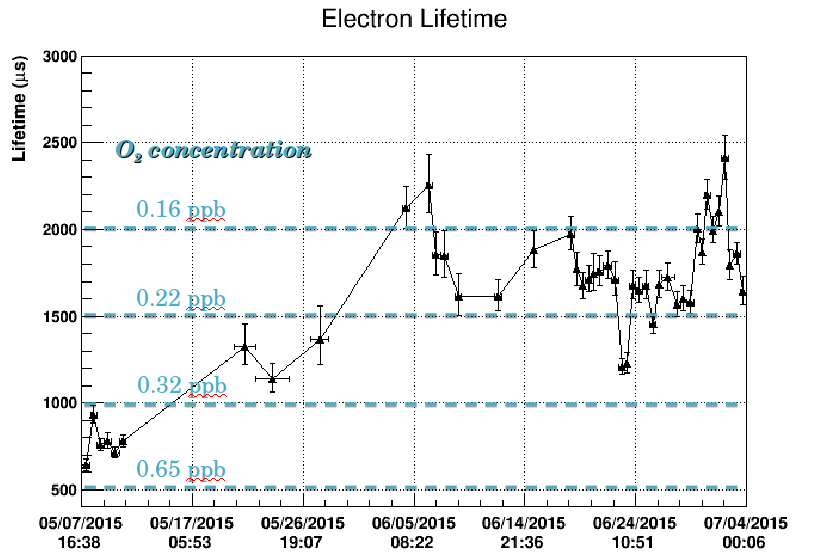
\includegraphics[scale=0.35]{./images/Run1Lifetime.png}
\includegraphics[scale=0.28]{./images/Run2Lifetime.png}
\caption{Electron lifetime for Run-I (Top) and Run-II (Bottom), obtained with the multi-track method (see DocDb 1804). Errors are statistical only.}
\label{fig:LifetimeNOchargecorrection}
\end{figure}

\paragraph{\textbf{Calorimetry Constant Tuning}}
The calorimetry constants used in this data analysis were determined from a sample of data and Monte Carlo spanning Run I and Run II. The calibration method, described in greater detail in \href{https://lartpc-docdb.fnal.gov:441/cgi-bin/ShowDocument?docid=2513}{docDB-2513}, is predicated on the Bethe-Bloch description of the mean rate of energy loss for various particle species. The basic idea of this calibration technique is to utilize a portion of a track within the LArTPC that has a well known momentum and particle species to measure the energy deposited per unit length (dE/dX) as recorded inside the TPC. Once a sample of particles dE/dX has been measured at various momentums, we then tune to calorimetry constants within the reconstruction software to align these measured values to match the theoretical ones.

Figure \ref{fig:dEdXvsMomentum} shows the calorimetry response for the $\pi, \mu, e$-High-Yield data sample used in this analysis. The selection method for this sample is to take each  track within the TPC that is uniquely matched to a wire-chamber track and use the measured momentum for that track. We require the track to be of a minimum length of 10~cm long (to ensure we are away from any interaction point where the track may be broken into subsequent tracks). We then take the first twelve spacepoints of the track (excluding the first point to avoid edge effects near the field cage) and sample the reconstructed dE/dX for each point along the track. On average, this samples 5~cm of the track and takes the dE/dX measurements are then put into a histogram that corresponds to measured momentum of the track.

\begin{figure}[h!]
\centering
\includegraphics[scale=0.33]{./images/dEdXvsMomentumCombined.png}
\includegraphics[scale=0.33]{./images/dEdXDataFit.png}
\caption{(LHS)dE/dX most probable value (MPV) as a function of momentum for the sample of events used in this analysis. (RHS) dE/dX for the sample used in this analysis fit with a Landau between 1.25 MeV/cm $<$ dE/dX $<$ 12 MeV/cm (similarly to what was done in the calibration procedure), returning a MPV of 1.589 MeV/cm. These values are obtained using the calorimetry constants derived in \href{https://lartpc-docdb.fnal.gov:441/cgi-bin/ShowDocument?docid=2513}{docDB-2513}}
\label{fig:dEdXvsMomentum}
\end{figure}

\newpage
%%%%%%%%%%%%%%%%%%%%%%%%%%%%%%%%%%%%%%%%%%%%%%%%%%%%%%%%%%%%
\subsubsection{Data/MC Comparisons} \label{sec:DataMCCompare}
%%%%%%%%%%%%%%%%%%%%%%%%%%%%%%%%%%%%%%%%%%%%%%%%%%%%%%%%%%%%

Here we present a series of low-level plots which validate the data and Monte Carlo reconstruction. Each set of plots is shown with the y-axis in both linear and log scale to allow for comparisons in the bulk as well as the tale. Commentary on any set of plots is made in the caption.

\begin{figure}[h!]
\centering
\includegraphics[scale=0.33]{./images/TrackPitch.png}
\includegraphics[scale=0.33]{./images/TrackPitchLog.png}
\caption{The reconstructed track pitch for data and Monte Carlo. Monte Carlo is scaled to data in the proportions which represent both the expected beam composition (Table \ref{tab:beamcomp1}) and the selection efficiency for that sample (Table \ref{tab:MCPercentageTable}. The data and MC agree well in the bulk of the sample, with the high end of the track pitch tail showing some disagreement, suggesting different pathologies in the data and MC cause points to be skipped along the track. These difference are quantitatively small and thus shouldn't impact the final result. }
\label{fig:DataMCTrackPitch}
\end{figure}

\begin{figure}[h!]
\centering
\includegraphics[scale=0.33]{./images/TrackLength.png}
\includegraphics[scale=0.33]{./images/TrackLengthLog.png}
\caption{The reconstructed track length for data and Monte Carlo. Monte Carlo is scaled to data in the proportions which represent both the expected beam composition (Table \ref{tab:beamcomp1}) and the selection efficiency for that sample (Table \ref{tab:MCPercentageTable}. The data and MC agree overall with the MC slightly over-predicting the shortest tracks where the electron and photon samples dominate. Later plots show these slight difference to be negligible to the overall analysis.}
\label{fig:DataMCTrackLength}
\end{figure}

\begin{figure}[h!]
\centering
\includegraphics[scale=0.33]{./images/dEdX.png}
\includegraphics[scale=0.33]{./images/dEdXLog.png}
\caption{The reconstructed energy deposited per unit length (dE/dX) for data and Monte Carlo. Monte Carlo is scaled to data in the proportions which represent both the expected beam composition (Table \ref{tab:beamcomp1}) and the selection efficiency for that sample (Table \ref{tab:MCPercentageTable}. The data and MC agree in the most probable value (MPV) and in the shape. There is a slight difference in the highest side tail for the dE/dX $>$ 6 MeV/cm. This corresponds to a very small overall component of the sample and thus should only cause a slight difference in the computation of the kinetic energy for the track.}
\label{fig:DataMCdEdX}
\end{figure}

\begin{figure}[h!]
\centering
\includegraphics[scale=0.33]{./images/dEdXvsRRData.png}
\includegraphics[scale=0.33]{./images/dEdXvsRRDataLog.png}
\caption{The reconstructed energy deposited per unit length (dE/dX) versus the Residual  Range for the data sample selected in Table \ref{tab:CutSummary}. These results agree well with Figure \ref{fig:PionMCdEdXvsRR} giving confidence that the sample of data is dominated by minimum ionizing particles (such as pions) and that the samples are well calibrated.}
\label{fig:DatadEdXvsRR}
\end{figure}

\begin{figure}[h!]
\centering
\includegraphics[scale=0.33]{./images/dEdXvsRRPionMC.png}
\includegraphics[scale=0.33]{./images/dEdXvsRRPionMCLog.png}
\caption{The reconstructed energy deposited per unit length (dE/dX) versus the Residual  Range for the Pion MC sample selected in Table \ref{tab:MCRunIICutSummary}.}
\label{fig:PionMCdEdXvsRR}
\end{figure}

\newpage
%%%%%%%%%%%%%%%%%%%%%%%%%%%%%%%%%%%%%%%%%%%%%%%%%%%%%%%%%%%%
\subsubsection{Energy Reconstruction Cross-Check} \label{sec:ERecoCrossCheck}
%%%%%%%%%%%%%%%%%%%%%%%%%%%%%%%%%%%%%%%%%%%%%%%%%%%%%%%%%%%%

Figure \ref{fig:RecoEvsTrueE} shows the reconstructed kinetic energy at the interaction point for a sample of $\pi^{-}$ MC compared to the true energy the pion had at the interaction point. The reconstructed energy at the interaction point is calculated by
\begin{equation}
KE_{Interaction} = \sqrt{P_{WCtrk}^2 + m_{\pi}^2} - E_{Loss} - (\Sigma dE/dX_{i} \times Pitch)
\end{equation}
where $P_{WCtrk}$ represents the momentum as simulated by the equivalent of the wire-chamber track in the MC, $m_{\pi}$ is the mass of the pion, $E_{Loss}$ is the flat energy correction which takes into account the energy loss due to the interviening material between WC-4 and the front face of the TPC (here assumed to be 40 MeV) and $\Sigma dE/dX_{i} \times Pitch$ is the energy loss using the reconstructed track. This shows very good agreement with a linear regression fit which returns a near diagonal line with a y-intercept close to zero.

\begin{figure}[htb]
\centering
\includegraphics[scale=0.38]{./images/RecoEvsTrueE.png}
\caption{Reconstructed kinetic energy at the interaction point for a sample of DDMC $\pi^{-}$ compared to the kinetic energy of the pion as calculated from Geant4. The plot is fit with a linear regression which returns an R$^{2}$ = 0.87 and a y intercept of -1.72 MeV with a slope of 0.94.}
\label{fig:RecoEvsTrueE}
\end{figure}

As a point of comparison, Figure \ref{fig:LengthRecoEvsTrueE} shows the reconstructed kinetic energy at the interaction point versus the true energy at the interaction point where instead of using the calorimetry tools we calculate the reconstructed energy using the length of the track. Here the reconstructed energy is given by 
\begin{equation}
KE_{Interaction} = \sqrt{P_{WCtrk}^2 + m_{\pi}^2} - E_{Loss} - (2.1 MeV/cm \times Length_{Reco})
\end{equation}
where 2.1 MeV/cm is the mean of the dE/dX distribution and $Length_{Reco}$ is the reconstructed length of the track up to its interaction point. This also gives good agreement with only a slight improvement on the linear regression fit as compared to the sample using the reconstructed calorimetry.
 
\begin{figure}[htb]
\centering
\includegraphics[scale=0.38]{./images/LengthRecoEvsTrueE.png}
\caption{Length based reconstructed kinetic energy at the interaction point for a sample of DDMC $\pi^{-}$ compared to the kinetic energy of the pion as calculated from Geant4. The plot is fit with a linear regression which returns an R$^{2}$ = 0.92 and a y intercept of -1.26 MeV with a slope of 0.95.}
\label{fig:LengthRecoEvsTrueE}
\end{figure}

For completeness, the calorimetry based method is compared to the length based method in Figure \ref{fig:CaloMethvsLengthMeth}. The two methods return very nearly to same answer over the range of kinetic energy seen in LArIAT. This gives us confidence in continuing to use the calorimetry based reconstruction of our kinetic energy as the method for calculating the cross-section as a function of kinetic energy.

\begin{figure}[htb]
\centering
\includegraphics[scale=0.38]{./images/CaloMethodsCompared.png}
\caption{(LHS) Length based kinetic energy versus the calorimetry based kinetic energy. (RHS) Calculated the $\Delta$E (True - Reco) for the two methods. Red: Length Based, Blue: Calorimetry Based. }
\label{fig:CaloMethvsLengthMeth}
\end{figure}



\newpage




\newpage
%%%%%%%%%%%%%%%%%%%%%%%%%%%%%%%%%
%%  BIBLIOGRAPHY	
%%%%%%%%%%%%%%%%%%%%%%%%%%%%%%%%%
%\begin{thebibliography}{99}
\footnotesize

%1
\bibitem{PDG}
PASSAGE OF PARTICLES THROUGH MATTER, . Nakamuraet al.(PDG), JP G37, 075021 (2010) and 2011 partial update for the 2012 edition \url{http://pdg.lbl.gov/2011/reviews/rpp2011-rev-passage-particles-matter.pdf}.

%2
\bibitem{PDG-Argon}
PDG Tables for Liquid Argon \url{http://pdg.lbl.gov/2017/AtomicNuclearProperties/MUE/muE_liquid_argon.txt}. 

\bibitem{WCTrackReco}
Wire Chamber Track Reconstruction, LArIAT DocDB 1771 \url{https://lartpc-docdb.fnal.gov:441/cgi-bin/ShowDocument?docid=1771}

\end{thebibliography}
\textbf{}
\begin{thebibliography}{99}
\footnotesize

%1
\bibitem{PDG}
PASSAGE OF PARTICLES THROUGH MATTER, . Nakamuraet al.(PDG), JP G37, 075021 (2010) and 2011 partial update for the 2012 edition \url{http://pdg.lbl.gov/2011/reviews/rpp2011-rev-passage-particles-matter.pdf}.

%2
\bibitem{PDG-Argon}
PDG Tables for Liquid Argon \url{http://pdg.lbl.gov/2017/AtomicNuclearProperties/MUE/muE_liquid_argon.txt}. 

\bibitem{WCTrackReco}
Wire Chamber Track Reconstruction, LArIAT DocDB 1771 \url{https://lartpc-docdb.fnal.gov:441/cgi-bin/ShowDocument?docid=1771}

\end{thebibliography}
\textbf{}



\end{document}